% mnras_template.tex
%
% LaTeX template for creating an MNRAS paper
%
% v3.0 released 14 May 2015
% (version numbers match those of mnras.cls)
%
% Copyright (C) Royal Astronomical Society 2015
% Authors:
% Keith T. Smith (Royal Astronomical Society)

% Change log
%
% v3.0 May 2015
%    Renamed to match the new package name
%    Version number matches mnras.cls
%    A few minor tweaks to wording
% v1.0 September 2013
%    Beta testing only - never publicly released
%    First version: a simple (ish) template for creating an MNRAS paper

%%%%%%%%%%%%%%%%%%%%%%%%%%%%%%%%%%%%%%%%%%%%%%%%%%
% Basic setup. Most papers should leave these options alone.
\documentclass[a4paper,fleqn,usenatbib]{mnras}
\usepackage[T1]{fontenc}
\usepackage{ae,aecompl}

% Only include extra packages if you really need them. Common packages are:
\usepackage{graphicx}	% Including figure files
\usepackage{amsmath}	% Advanced maths commands
\usepackage{amssymb}	% Extra maths symbols
\usepackage{subfig}
\usepackage{array}

% Included by user
\usepackage{multirow}
\usepackage{multicol}
\usepackage{blindtext}
\newcolumntype{?}{!{\vrule width 1pt}}

\newenvironment{Table}
   {\par\bigskip\noindent\minipage{\columnwidth}\centering}
   {\endminipage\par\bigskip}
%%%%%%%%%%%%%%%%%%%%%%%%%%%%%%%%%%%%%%%%%%%%%%%%%%

%%%%% AUTHORS - PLACE YOUR OWN COMMANDS HERE %%%%%

% Please keep new commands to a minimum, and use \newcommand not \def to avoid
% overwriting existing commands. Example:
%\newcommand{\pcm}{\,cm$^{-2}$}	% per cm-squared

%%%%%%%%%%%%%%%%%%%%%%%%%%%%%%%%%%%%%%%%%%%%%%%%%%

%%%%%%%%%%%%%%%%%%% TITLE PAGE %%%%%%%%%%%%%%%%%%%

% Title of the paper, and the short title which is used in the headers.
% Keep the title short and informative.
\title[MW DM halo shape in AURIGA]{The expected shape of the Milky Way's Dark Matter halo}

% The list of authors, and the short list which is used in the headers.
% If you need two or more lines of authors, add an extra line using \newauthor
\author[Jesus Prada,  Jaime E. Forero-Romero, Volker Springel ]{
Jesus Prada,$^{1}$\thanks{E-mail: jd.prada1760@uniandes.edu.co}
Jaime E. Forero-Romero,$^{1}$
Volker Springel$^{2}$
\\
% List of institutions
$^{1}$Departamento de F\'sica, Universidad de los Andes, Cra. 1 No.
18A-10, Edificio Ip, Bogot\', Colombia.\\
$^{2}$Heidelberg Institute for Theoretical Studies, Schloss-Wolfsbrunnenweg 35, D-69118 Heidelberg
Germany.\\
}

% These dates will be filled out by the publisher
\date{Accepted XXX. Received YYY; in original form ZZZ}

% Enter the current year, for the copyright statements etc.
\pubyear{2018}

% Don't change these lines
\begin{document}
\label{firstpage}
\pagerange{\pageref{firstpage}--\pageref{lastpage}}
\maketitle

% Abstract of the paper
\begin{abstract}
We measure the shape of the dark matter halos of Milky Way type galaxies.
\end{abstract}

% Select between one and six entries from the list of approved keywords.
% Don't make up new ones.
\begin{keywords}
keyword1 -- keyword2 -- keyword3
\end{keywords}

%%%%%%%%%%%%%%%%%%%%%%%%%%%%%%%%%%%%%%%%%%%%%%%%%%

%%%%%%%%%%%%%%%%% BODY OF PAPER %%%%%%%%%%%%%%%%%%

\section{Introduction}


A robust prediction of the Cold Dark Matter (CDM) paradigm is that DM
halos are ellipsoidal and can be characterized by the principal axes
$a>b>c$.
This ellipsoidal shape is mostly due to the anisotropical and
clumpy accretion of matter influenced by environmental structures.
Numerical studies how that the shape has a strong mass dependence
\citep{Allgood_et_al._2006}, halos are also rounder at the outerskirts
than at the inner part. 
Shape also evolves with cosmic time, halos get
rounder as they evolve.  

There is however a high degree of uncertainty on what is the degree of
uncertainty on the degree of ellipticity of the Milky Way DM halo.
This problem has been addressed both by observations and simulations.
The difficulty in making an observational measurement lies in the
indirect nature of the effect; i.e. the ellipticity can only be
constrained by its effects on quantities such as stellar radial
velocities.
In simulations the uncertainty on predicting the MW DM ellipticity is 
driven by the different physical effects that should be modeled and
its different possible numerical implementations.


Observationally some studies prefer oblate (i.e. a=b>c) configurations at small
distances around $\leq 20$ kpc
\citep[see][]{Law_and_Majewski_2010,Bovy_et_el._2016,Loebman_et_al._2012,Olling_and_Merrifield_2000,Banerjee_and_Chanda_2011} 
and more triaxial and prolate configurations on the outter distances
$\geq 20$ kpc 
\citep[see][]{Vera-Ciro_and_Helmi_2013,Law_and_Majewski_2009,Deg_and_Widrow_2013,Banerjee_and_Chanda_2011}.
However, some  studies are inclined towards prolate configurations even at the inner
parts of the halo \citep[see][]{Bowden_et_al._2016}, and
although it previously seemed that a triaxial DM halo on the
outerskirts would be necessary to fully explain the characterization
of the Sagittarius stream \citep{Law_and_Majewski_2009}, recent studies
questioned this claim by reporting inconsistencies with narrow stellar
streams \citet{Pearson_et_al._2015} or finding that
the relaxation of other constraints may make this claim unnecessary
\citet{Ibata_et_al._2013}. 

In simulations there is strong evidence claiming that the presence of
baryons produces axisymmetrical halos.  
For instance, some studies have shown that the DM halo shape must be
axisymmetrical to ensure the stability of a hydrodynamical disk
embeded in a static DM halo. 
Other have studied this rounding effect by simulating the disk as rigid
potential inside an N-body triaxial DM
halo \cite{Debattista_et_al._2008,Debattista_et_al._2013,Kazantzidis_et_al._2010}
finding that the halo responds to the disk by becoming less triaxial. 

The caveat of the studies mentioned above is that they do not
follow baryons in the whole cosmological context. 
Other studies overcome this limitation by using resimulations 
\citep{Abadi_et_al._2010,Bryan_et_al._2013} finding that the
feeback related to star formation in the disk drives the strenght of
the round effect. 
Recently \cite{2018arXiv180907255C} made a study in a cosmological
simulation to compare the effect of including baryons. They do find,
on average, rounder halo shapes once hydrodynamic effects are
included, but it is uncertain the strenght of this statistical effect
on galaxies similar to the MW.


All these difficulties (enough numerical resolution, explicit
cosmological context, appropriate feedback physics to produce
realistic MW disks) have limited the studies that want to study the
rounding effect of baryons in MW-like galaxies.
In this work we overcome all these limitations by analyzing the
results of state-of-the-art hydrodynamical simulations of isolated
halos that resemble the Milky Way.
We also perform a convergence study with simulation performed at
different resolution levels and explicitly compare the role of DM only
vs. DM+hydro on the MW DM halo shape.


%\begin{multicols}{2}
\begin{table*}
%\setlength{\tabcolsep}{3pt}
\begin{tabular}{|l|cc|cc|c|c|p{4cm}|}\hline
Reference&$q_{\rho}$&$s_{\rho}$&$q_{\phi}$&$s_{\phi}$&$R$&$\theta$&comment\\ \hline \hline
\citet{Olling_and_Merrifield_2000}& $\mathbf{1.00}$ & $\mathbf{0.80}$ & & & $\simeq 8$kpc & $0^{\circ}$&Method: Stellar dynamics and HI density. \\\hline
\citet{Law_and_Majewski_2009}&&&$\mathbf{0.83}$&$\mathbf{0.67}$& $\lesssim 60$kpc&$90^{\circ}$&Mid-axis orientation. Method: Sagittarius stream\\\hline
%
\citet{Law_and_Majewski_2010}&&&$\mathbf{0.99}$&$\mathbf{0.72}$& $[20$kpc,$60$kpc$]$&$90^{\circ}$&Mid-axis orientation, Method: Sagittarius stream\\\hline
%
\citet{Loebman_et_al._2012}&$\mathbf{1.00}$&$\mathbf{0.47}$&&&$\sim 20$kpc &$0^{\circ}$&Method: SDSS statistics\\\hline
%
\citet{Deg_and_Widrow_2013}&$0.72$&$0.28$&$0.82$&$0.40$&$[20$kpc,$60$kpc$]$&$90^{\circ}$& Mid-axis orientation. Method: Sagittarius stream\\\hline
%
\multirow{2}{*}{\citet{Vera-Ciro_and_Helmi_2013}}&&&$\mathbf{1.00}$&$\mathbf{0.90}$&$\lesssim 10$kpc&$0^{\circ}$ & Method: Sagittarius stream \& LMC \\
&&&$\mathbf{0.90}$&$\mathbf{0.80}$&$\gtrsim 10$kpc&$90^{\circ}$& Mid-axis orientation on the outside. \\\hline
%
\citet{Bovy_et_el._2016}&$\mathbf{0.95}$&$\mathbf{0.95}$&&&$\lesssim 20$kpc&$90^{\circ}$ & Method: Stellar streams\\\hline
%
\citet{Bowden_et_al._2016}&&&$\mathbf{[0.5,0.66]}$&$\mathbf{[0.5,0.66]}$&$[5$kpc,$10$kpc$]$&$90^{\circ}$& Weak constraint on prolate halo. Method: SDSS stars dynamics.\\\hline
%
\multirow{2}{*}{\citet{Banerjee_and_Chanda_2011}}&$\mathbf{1}$&$\mathbf{1}$&&&$9$kpc&$0^{\circ}$&Method: HI gas. \\
&$\mathbf{0.5}$&$\mathbf{0.5}$&&&$24$kpc&$0^{\circ}$&Monotonical change between radial regimes.\\\hline
%
\cite{Johnston_et_al._2005}&$\mathbf{1}$&$\mathbf{[0.83-0.92]}$&&&$\lesssim 60$kpc&$0^{\circ}$&Method: Sagittarius stream\\\hline\hline
\end{tabular}
\caption{(TODO: compute analogues in isopotential or isodensity according to Binney and Tremaine)}
\end{table*}
%\end{multicols}

\begin{table*}
%\setlength{\tabcolsep}{3pt}
\begin{tabular}{|l|cc|cc|c|p{4cm}|}\hline
Reference&$q_{\rho}$&$s_{\rho}$&$q_{\phi}$&$s_{\phi}$&$R$&comment\\ \hline \hline
\citet{Chua_et_al._2018}&$\mathbf{0.88\pm0.10}$&$\mathbf{0.70\pm0.11}$&&&$0.15R_{200}$& Illustris\\\hline
%
\citet{Bryan_et_al._2013}&$\mathbf{[0.84,0.86]}$&$\mathbf{[0.66,0.70]}$&&&$R_{200}$& For different cosmologies and feedback recipies. Calculated from a fit at $M_\odot=10^12$\\\hline
%
\multirow{2}{*}{\citet{Abadi_et_al._2010}}&&&$\mathbf{0.98}$&$\mathbf{0.85}$&-& Almost independent of radius. No feedback: boundary case\\\hline
\end{tabular}
\caption{(TODO: compute analogues in isopotential or isodensity according to Binney and Tremaine)}
\end{table*}




\section{Numerical Simulations}

In this work we use the results of the state-of-the art Auriga
simulations \citep{auriga}. 
The objects in those simulations were selected from a set of 30 isolated halos in
the Evolution and Assembly of GaLaxies and their Environments (EAGLE)
project \citep{Eagle}. 
These halos were randomly selected from a sample of the most isolated
quartile of halos whose virial mass $M_{200}$ varied between
$10^{12}M_\odot$ and $2\times 10^{12}M_\odot$. 
These halos were re-simulated with higher resolution an varying
physical realism using the AREPO code \citep{arepo}.
 
All 30 halos were simulated within resolution defined for Aquarius
simulations corresponding to $\sim 3\times 10^6$ high resolution DM
particles of $\sim 2.5 \times 10^5 M_\odot$.  
This resolution is labeled as Level 4, the main details for each halo
are consigned in Table \ref{tab:level4}. 
From these 30 halos, 6 of them where re-simulated at higher resolution
(labeled as Level 3) taking into account a spatial factor of 2 in each
dimension.   
Details of Level 3 halos are in Table \ref{tab:level3}. 
Furthermore, for each halo in each level of resolution there are two
versions of the simulation: DM-only and DM plus baryons with
magneto-hydrodynamical (MHD) physics.  



\section{Determining the halo shape}

%\subsection{The solid ellipsoid method}

There are two main ways to estimate the DM halo shape at a fixed
radius: by computing isopotential or isodensity surfaces.
Observational inference models estimate the shape from the
isopotential contours, while simulations work with the isodensity
contours which can be  directly calculated from particle positions.  
However, the density contours are not smooth and are very 
sensitive to the presence of small satelites.
For this reason we choose to measure the shape by taking
volume-enclosed particles, rather than shell-enclosed.  

We follow the shape measurement method presented by
\cite{Allgood_et_al._2006} that uses the reduced
inertia tensor,     

\begin{equation}
I_{ij} = \sum_k \frac{x_k^{(i)}x_k^{(j)}}{d^2_k},
\label{eq:inertia}
\end{equation}

with the positions components weighted by the k-th particle distance
$d_k^2=x_k^2+y_k^2+z_k^2$, the particle positions are measured from
the minimum of the gravitational potential in each halo.
The diagonalization of this tensor yields the principal axes of the
structure as well as the eigen-quantities which are proportional to
the squared principal axes $a>b>c$. 

We start the calculations taking into account particles within a
sphere of radius $R$ and then  recharacterize the triaxial parameters by taking into account
particles within an ellipsoid of semi-axes $r,r/q,r/s$ and weighted
distance $d^2=x^2+(y/q)^2+(z/s)^2$, where $q = b/a$ and $s=c/a$
are the previously calculated axial ratios. 
We repeat this process until the average deviation of semi-axes is
less than $10^{-6}$.  
This is the same method used to estimate the halo shape in the DM-only
Aquarius simulations \citep{Vera-Ciro_et_al._2011}. 

We restrict the sampling of the ellipsoidal parameters to radii
between $1/16 R_{vir}$ and $2R_{vir}$, where  $R_{vir}$ is taken as the
radius enclosing a sphere with 500 times the average dark matter
density of the Universe. All our results use of this reference radius
unless strictly stated otherwise. 
We peform the shape measurements both as a function of radius and
redshift for all halos in the sample.


\section{Results}

\subsection{Radial trends}


In DM-only simulations halos are monotonically rounder with increasing
radius, this confirms results already reported in the literature
\citep{Vera-Ciro_et_al._2011}. 
Figure \ref{fig:slices} illustrates this effect.
There we show the DM density of a DM-only halo at redshift zero.
The halo is aligned with the minor axis. 
The ellipsoid shows the outermost boundary of the estimated shape ellipsoid.
Formally, this effect is reflected in the axial ratios $b/a,c/a$, which tend to unity
on the outerskirts of the halo. As a representative sample of this
relations, we show on figure \ref{fig:DM relation} the evolution, for
a specific halo, of the axial ratios $b/a,c/a$ and the triaxiality
parameter $T=\frac{a^2-b^2}{a^2-c^2}$ in a wide range of radii. 


\begin{figure*}
  \centering
  \subfloat[halo 27 DM shape at small radius]{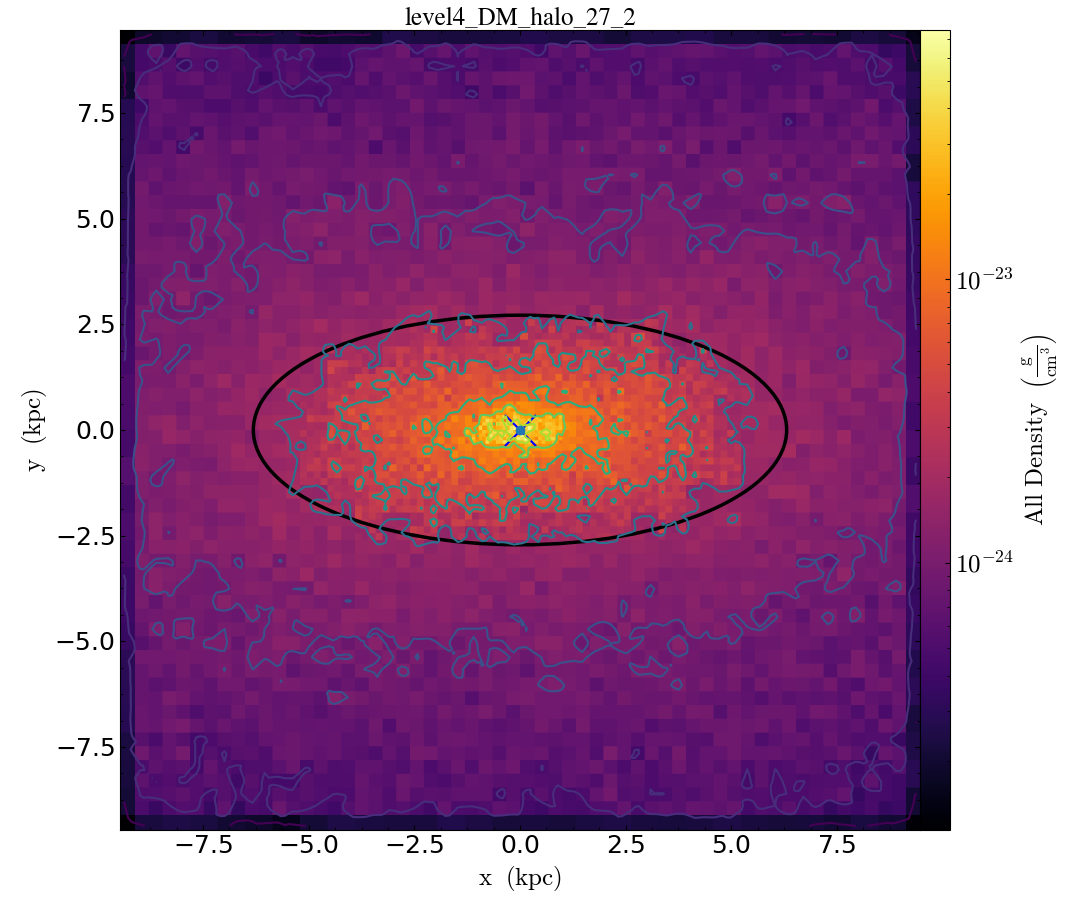
\includegraphics[width=0.5\textwidth]{./pics/MHD_Vs_DM/level4_DM_halo_27_inner.png}}
  \hfill
  \subfloat[halo 27 DM shape at big radius]{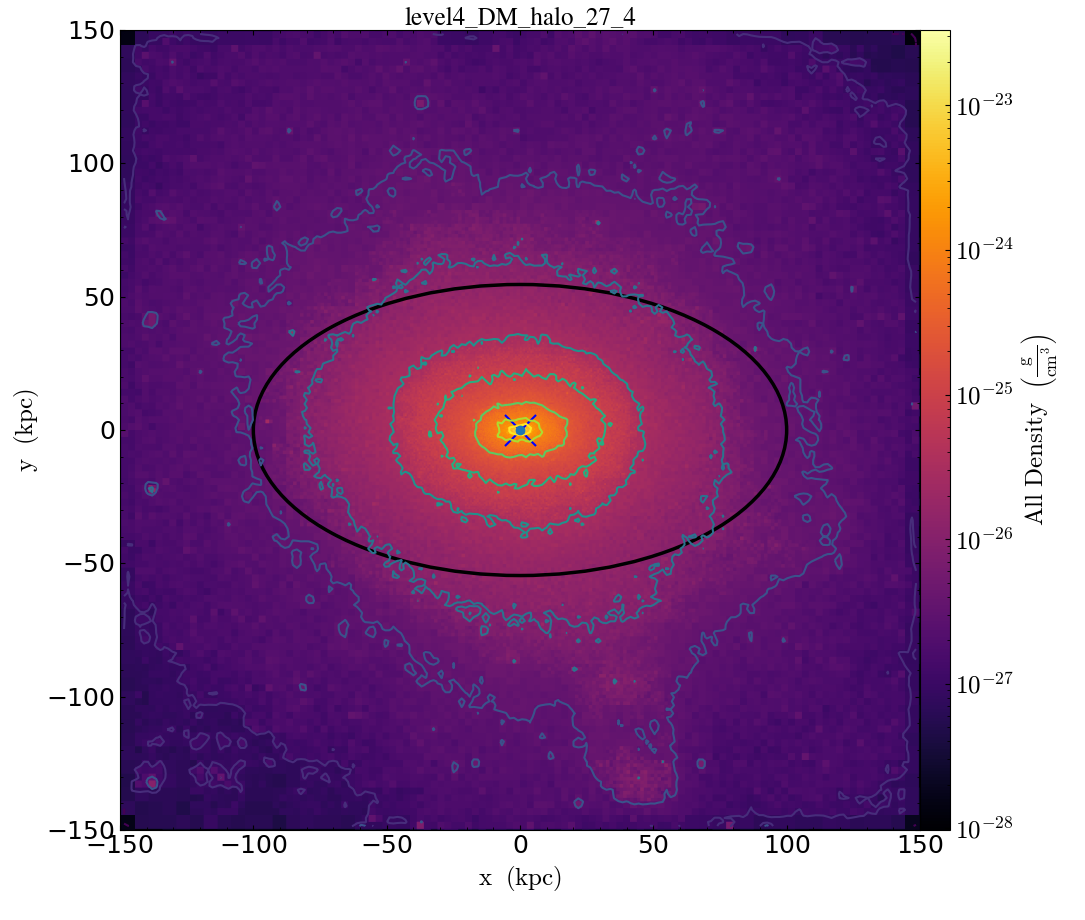
\includegraphics[width=0.5\textwidth]{./pics/MHD_Vs_DM/level4_DM_halo_27_outter.png}}
  \hfill
  \caption{DM density for inner/outer (left/right panel) DM halo regions.}
  \label{fig:slices}
\end{figure*}

 \bibliographystyle{mnras}
 \bibliography{references}
\end{document}



\subsection{The radial tendency of axial ratios}



We found that most halos exhibit a monotonically-increasing somewhat
steady tendency of its axial ratios $b/a,c/a$  with radius, which is
well exemplified on figure \ref{fig:DM_MHD}. There are some special
cases in which fluctuations of the local DM density field affects this
relation, but in average, this monotonic and steady tendency is clear
and can be consulted on table \ref{table:DM table}. To ilustrate the
average behavior, as well as some peculiarities, we resume the results
of the 30 auriga simulations on the figure \ref{fig:Triax_DM} where
each shape represents a point in the triaxiality plane $c/a$ Vs
$b/a$. Check Vera-ciro onthis. 

\begin{figure}
\centering
{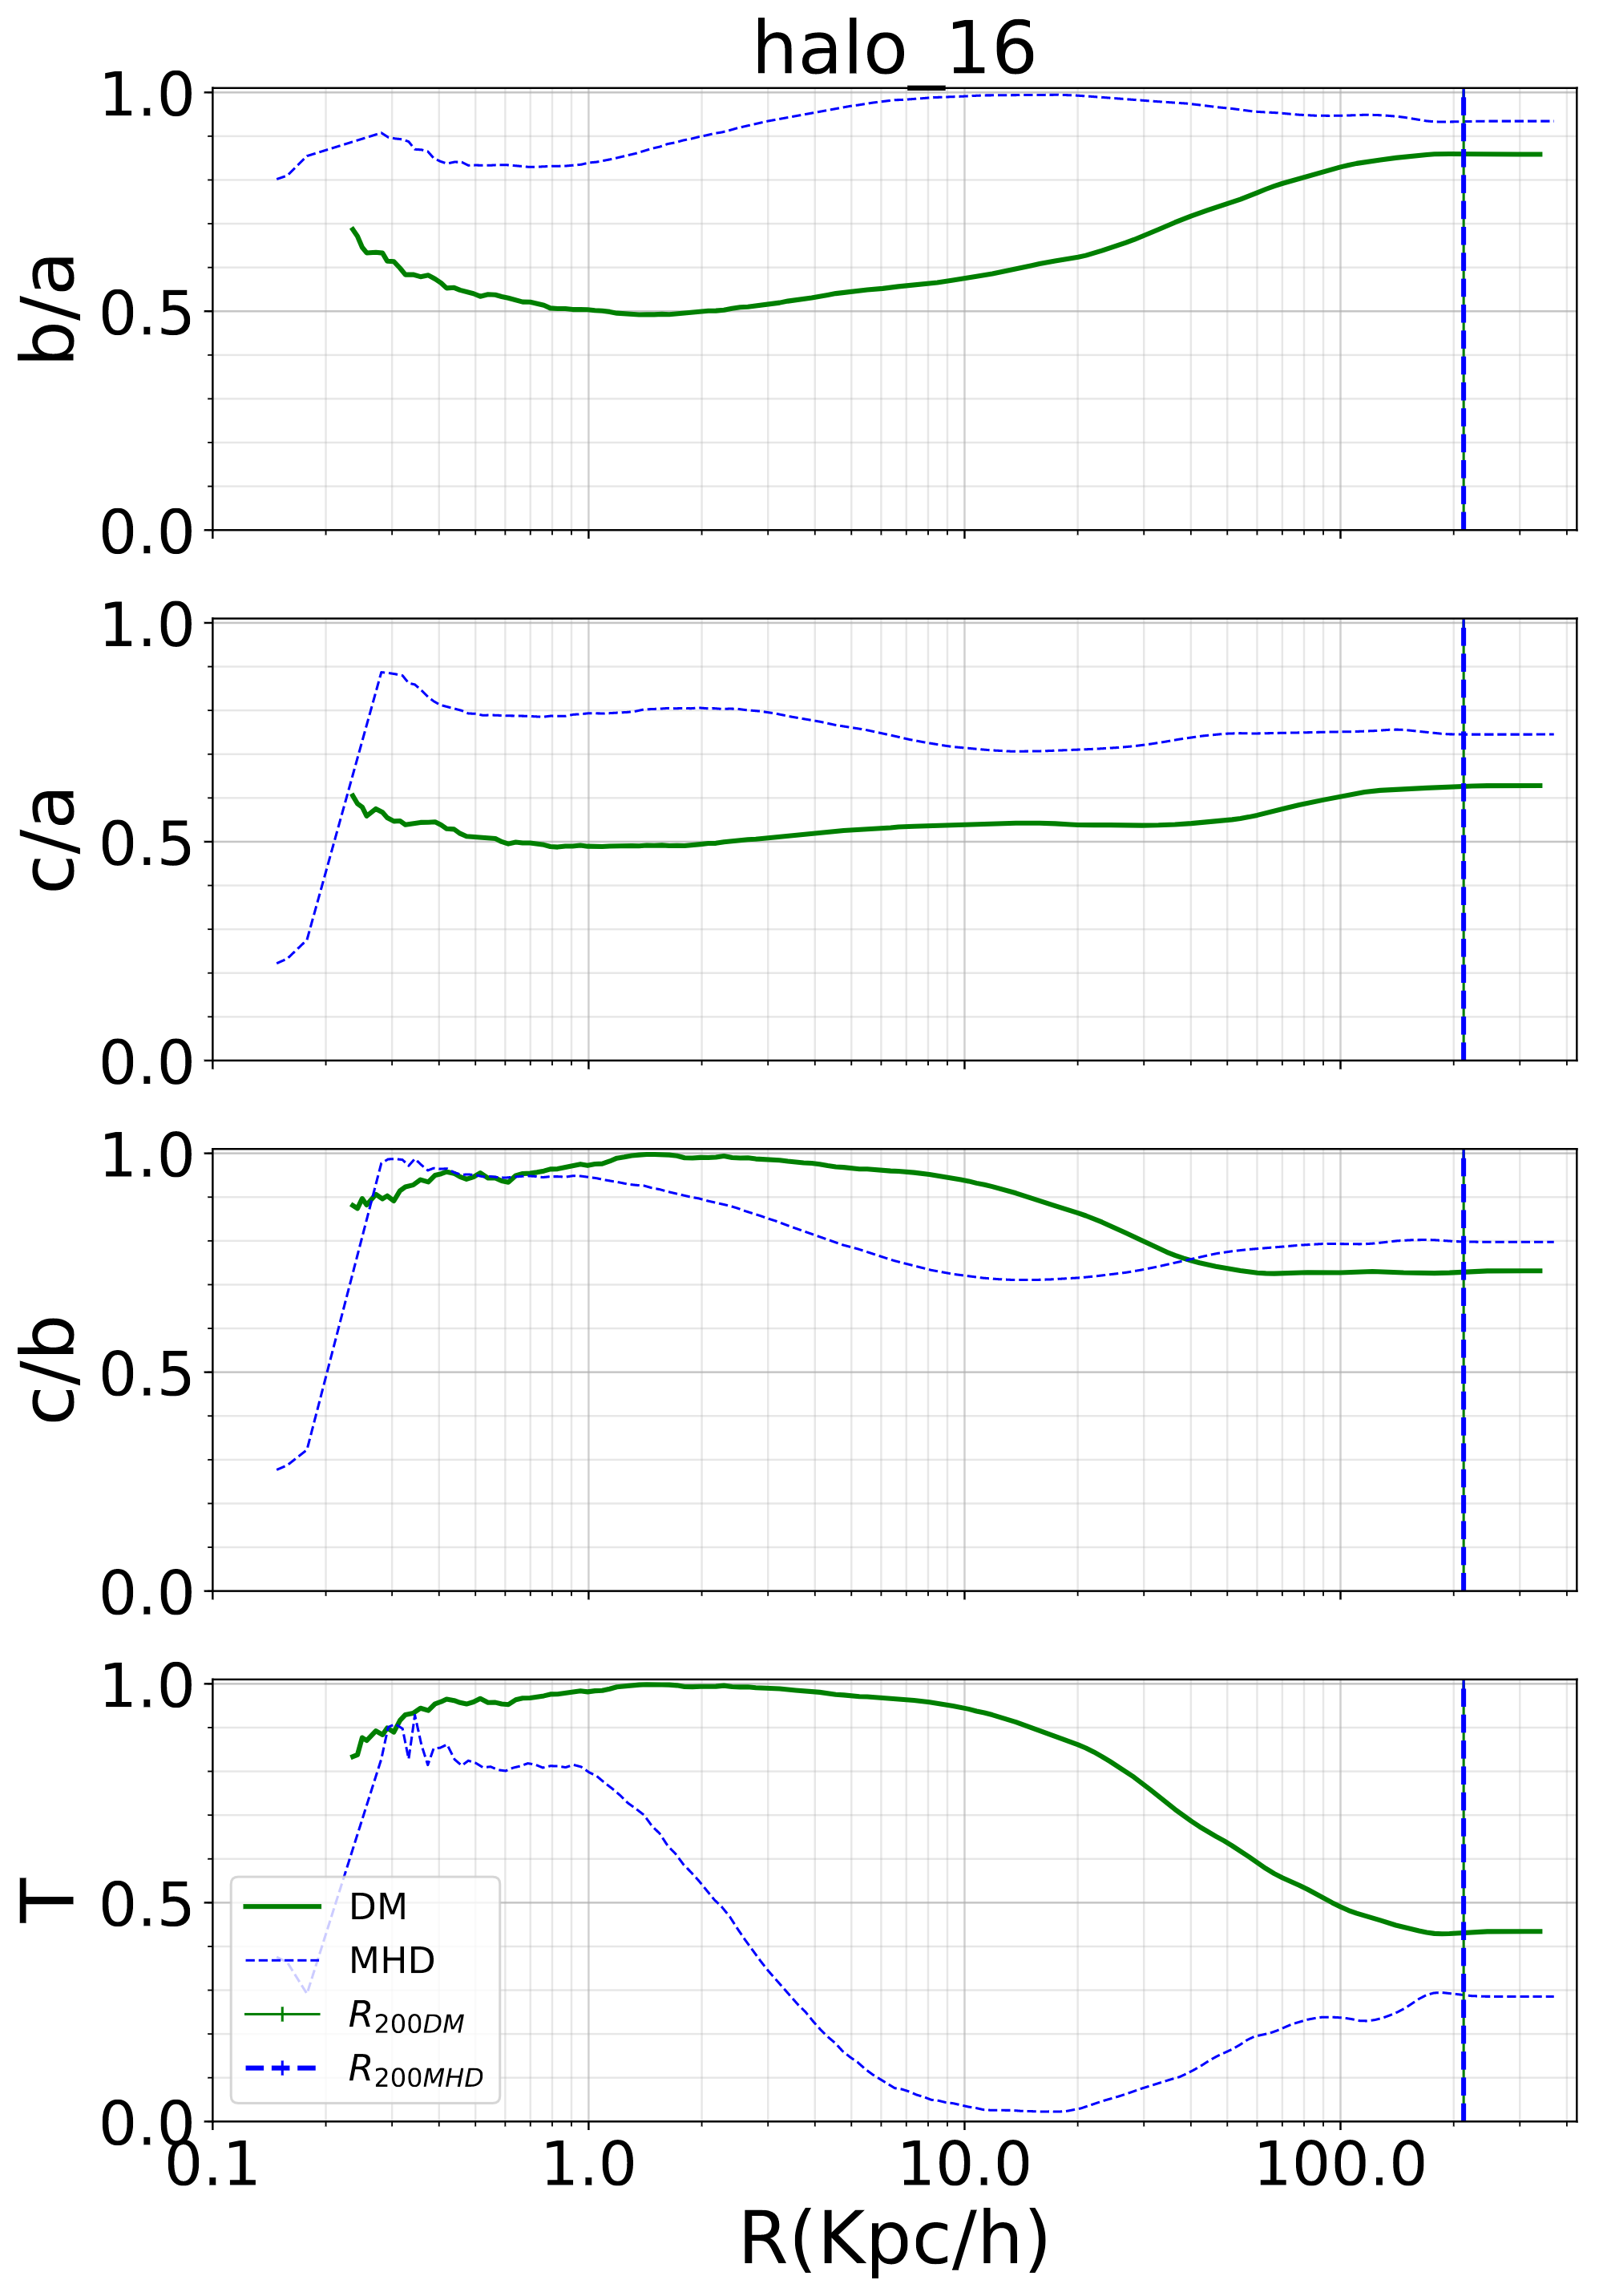
\includegraphics[width=0.8\columnwidth]{./pics/halo16.png}}
\caption{Radial profile for axial ratios and the triaxiality parameter $T=\frac{1-b/a}{1-c/a}$ for halo 16.}
\label{fig:DM_MHD}
\end{figure} 

 
\begin{figure}
  \centering
 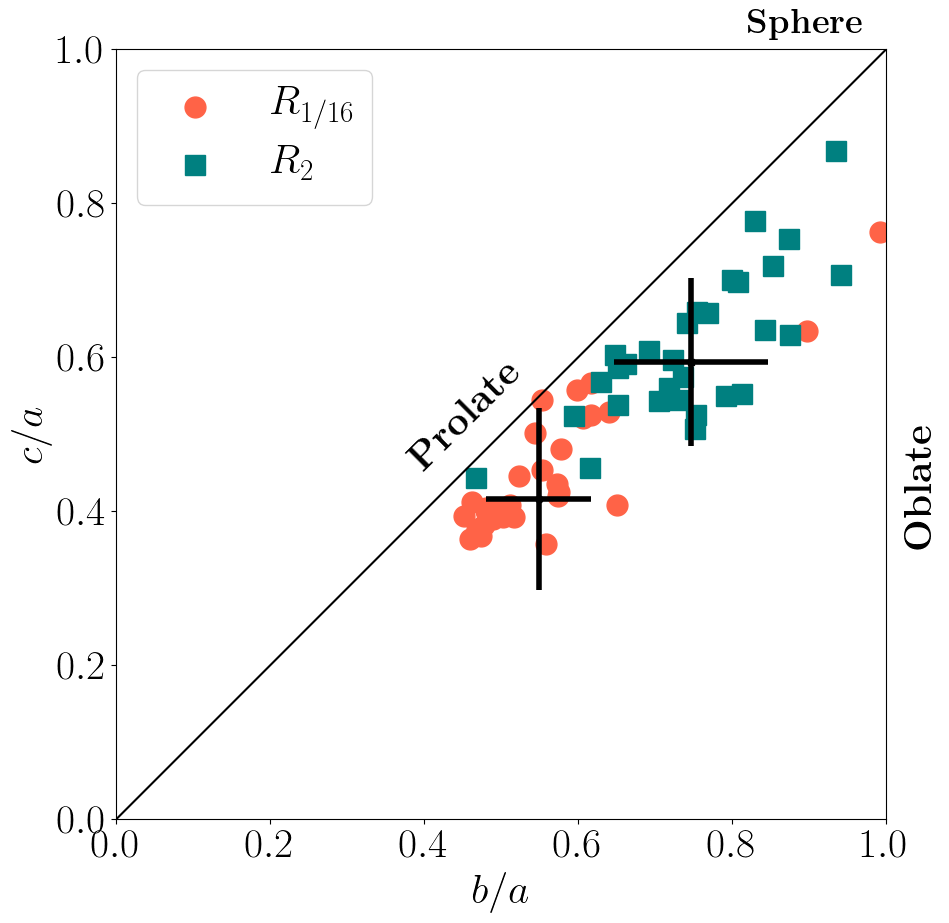
\includegraphics[width=0.9\columnwidth]{./pics/Triaxial_Plane/Triax_DM.png}
  
  \hfill
  \caption{Shape of each halo on the plane $c/a$ Vs $b/a$. Errorbar shows median and errors for each sampled radii. }
  \label{fig:Triax_DM}
\end{figure}

\begin{table}
\setlength{\tabcolsep}{3pt}
\begin{tabular}{l|cccccc}
 &$R_{1/16}$& $R_{1/8}$& $R_{1/4}$& $R_{1/2}$& $R_1$ & $R_2$\\
\hline \hline
$\bar{q}$&$0.55^{+0.07}_{-0.07}$&$0.57^{+0.09}_{-0.08}$&$0.61^{+0.15}_{-0.08}$&$0.65^{+0.18}_{-0.10}$&$0.70^{+0.13}_{-0.10}$&$0.75^{+0.10}_{-0.10}$ \\ [0.1cm]
$\bar{s}$&$0.42^{+0.12}_{-0.03}$&$0.45^{+0.11}_{-0.04}$&$0.49^{+0.09}_{-0.05}$&$0.52^{+0.10}_{-0.05}$&$0.56^{+0.10}_{-0.05}$&$0.59^{+0.11}_{-0.06}$ \\ [0.1cm]
$\bar{T}$&$0.89^{+0.03}_{-0.08}$&$0.88^{+0.04}_{-0.12}$&$0.84^{+0.08}_{-0.23}$&$0.81^{+0.08}_{-0.29}$&$0.75^{+0.14}_{-0.25}$&$0.71^{+0.16}_{-0.19}$ \\ [0.1cm]

\hline
\end{tabular}
\caption{Median values of axial ratios $q,s$ and triaxiality parameter $T$ for DM halos in DM-only simulations at different radii (columns). }
\label{tabe:DM table}
\end{table}

Concerning MHD halos, \textit{prescindible?(((the expected tendency is
  not clear. Some studies claim that the DM halo must be oblate, at
  least in the vicinities of the disk, to ensure its stability
  \cite{disk stability}. However,)))} not much is said about its
dependence with radius as previous studies focus rather on the effects
of baryons on the dynamics of the halo at fixed radii. Examining the
representative behaviour of a MHD halo on figure \ref{fig:DM_MHD},
some things are noticeable: first, the DM halo is almost perfectly
oblate around $\approx 10-30$Kpc, second, its axial ratio $b/a$ start
decreasing very slowly after $50Kpc$ and below $10Kpc$ and third, its
axial ratio $c/a$ does not exhibit noticeable change in the whole
radial domain. (Pass from representative case to averaged values)
These results are statistically supported and sumarized on table
\ref{MHD table} and figure \ref{fig:Triax_MHD} 

\begin{figure}
  \centering
 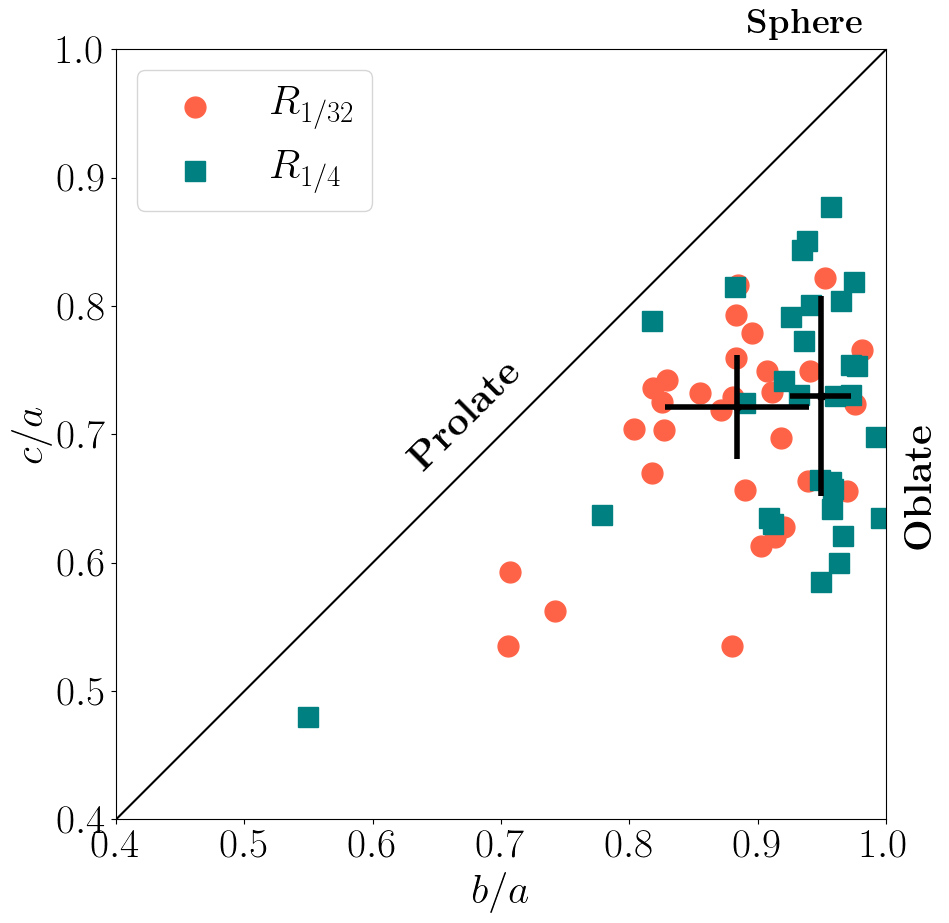
\includegraphics[width=0.9\columnwidth]{./pics/Triaxial_Plane/Triax_MHD.png}
  \hfill
  \caption{Shape of each halo on the plane $c/a$ Vs $b/a$. Errorbar
    shows median and errors for each sampled radii. } 
  \label{fig:Triax_MHD}
\end{figure}


\begin{table}
\setlength{\tabcolsep}{3pt}
\begin{tabular}{l|cccccc}
 &$R_{1/16}$& $R_{1/8}$& $R_{1/4}$& $R_{1/2}$& $R_1$ & $R_2$\\
\hline \hline
$\bar{q}$&$0.93^{+0.04}_{-0.04}$&$0.95^{+0.03}_{-0.03}$&$0.95^{+0.02}_{-0.05}$&$0.93^{+0.04}_{-0.06}$&$0.93^{+0.04}_{-0.10}$&$0.92^{+0.03}_{-0.09}$ \\[0.1cm]
$\bar{s}$&$0.73^{+0.05}_{-0.09}$&$0.73^{+0.07}_{-0.10}$&$0.73^{+0.08}_{-0.10}$&$0.73^{+0.09}_{-0.08}$&$0.75^{+0.07}_{-0.11}$&$0.74^{+0.07}_{-0.10}$ \\[0.1cm]
$\bar{T}$&$0.31^{+0.15}_{-0.22}$&$0.20^{+0.24}_{-0.12}$&$0.24^{+0.20}_{-0.12}$&$0.30^{+0.26}_{-0.16}$&$0.36^{+0.23}_{-0.23}$&$0.39^{+0.26}_{-0.13}$ \\[0.1cm]
\hline
\end{tabular}
\caption{Median values of axial ratios $q,s$ and triaxiality parameter $T$ for DM halos in MHD simulations at different radii (columns). }
\label{tabe:MHD table}
\end{table}

\subsection{Comparison with observational constraints}
To be able to compare our results with observational values, we must relate the calculated quanties with their corresponding isopotential analogue, in which observational constraints are usually presented. For this purpose, we run a simple algorithm to find an approximation of the shape of the isopotential contour. Here, we calculate the mean and standard deviation of the potential over a spherical shell of width equals to $10\%$ of the radius at which it is sampled. Then, we calculate the inertia tensor of particles with potential within $1\sigma$ around the mean potential and calculate its triaxial characterization with the reduced inertia tensor. We repeat the process of calculating the potential mean and standard deviation until convergence is achieved with tolerance of $10^{-4}$. We repeat this process for the different radii from table \ref{tabe:isopotential}. \\

\begin{table}
\setlength{\tabcolsep}{3pt}
\begin{tabular}{l|cccc}
 & $R_{1/8}$& $R_{1/4}$& $R_{1/2}$& $R_1$ \\
\hline \hline
$\bar{q}$&$0.98^{+0.01}_{-0.02}$&$0.97^{+0.01}_{-0.04}$&$0.96^{+0.03}_{-0.06}$&$0.94^{+0.03}_{-0.07}$ \\[0.1cm]
$\bar{s}$&$0.89^{+0.04}_{-0.06}$&$0.88^{+0.04}_{-0.04}$&$0.87^{+0.05}_{-0.05}$&$0.85^{+0.05}_{-0.05}$ \\[0.1cm]
$\bar{T}$&$0.18^{+0.23}_{-0.10}$&$0.36^{+0.19}_{-0.21}$&$0.40^{+0.26}_{-0.20}$&$0.48^{+0.23}_{-0.21}$ \\[0.1cm]
\hline
\end{tabular}
\caption{Median values of isopotential axial ratios $q,s$ and triaxiality parameter $T$ for DM halos in MHD simulations at different radii (columns). }
\label{tabe:isopotential}
\end{table}

As a check of consistency, we compare our new isopotential shape
results with the analytic expression of the
$(1-q_{\phi})\frac{1}{3}(1-q_{\rho})$ \citep[Binney and Tremaine
  year]{Binney and tremaine}, taking the volume-enclosed axial ratios
as an approximation for the isodensity contour ratios
$q_{\rho}$. Although this analytic expression if meant to be used for
logarithmic axisymmetric halos, it works well as a first approximation
for nearly axisymmetric halos as those produced by our disced
galaxies. We find that the difference between the real and the
analytic isopotential axial ratios is not bigger than $quantity
percent$. With this, we may now present on table
\ref{tabe:isopotential} our observationally-comparable results for MHD
halos at two important radii one corresponding to the approximate
regimes where the MW DM halo is usually constrained. 

Little discussion: Are our results congruent with observations? at
which radii, does the DM halo shape vary that much?. Which models are
favored? 


\subsection{The rounding effect of baryons}

From the previous characterization of radial shapes it is clear that
MHD halos are rounder than DM halos (i.e. axial ratios are bigger) at
every sampled radii. This can be compared on tables \ref{tabe:DM
  table} and \ref{tabe:MHD table} or at the representative example on
figure \ref{fig:DM_MHD}. From there, it is also noticeable that the
rounding effect of baryons is stronger at the disk regime, where the
DM halo is almost perfectly oblate. Furthermore, MHD halos tend
towards more oblate shapes (T < 0.5) despite DM halos tendency towards
more prolate shapes (T>0.5). 

This rounding effect is expected from the gravitational effect of the
flattened axisymmetric galactic disk. It is also reasonable that this
effect is not as strong at $\approx 100$Kpc, where the disk potential
is dimmer compared to the DM halo potential. Keeping this in mind, one
would expect that the rounding effect of baryons is related to some
galactic parameters such as its component masses and radii. However,
even for the parameter of highest correlation with this rounding
effect (the baryonic fraction), the relation is not clear nor
conclusive due to the dispersion from galaxy peculiarities. In figure
\ref{fig:Star_Density_effect} we plot the ratios $c/a$ compared to the
baryonic fraction of each galaxy. Although some linear tendency is
suggested qualitatively, the dispersion of the sample is very high to
obtain some conclusive relation. This is an evidence that
adiabatic-contraction models are not realistic as they may neglect
some effects of the galaxy evolution in the whole cosmological
context.  

\begin{figure}
	% To include a figure from a file named example.*
	% Allowable file formats are eps or ps if compiling using latex
	% or pdf, png, jpg if compiling using pdflatex
	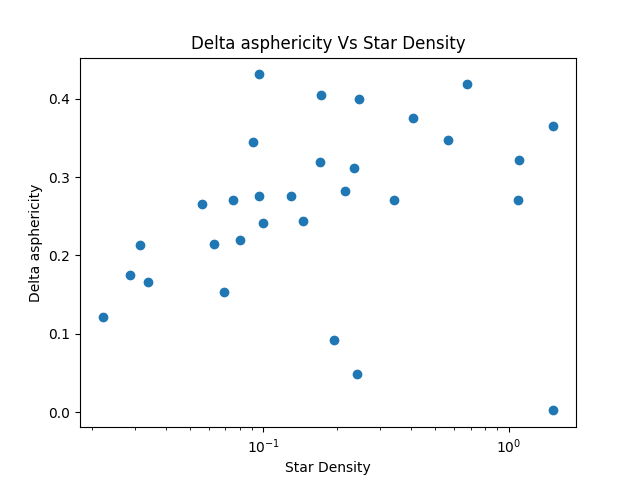
\includegraphics[width=\columnwidth]{./pics/Delta asphericity Vs Star Density.png}
    \caption{Difference in asphericities between MHD and DM shapes Vs Star Density of the simulation.}
    \label{fig:Star_Density_effect}
\end{figure}

\textbf{Actually we have not examined the relation of c/a in MHD halos
  with some measure of c/a from the disk, that is something like
  Zdisk/Rdisk. This actually would make more sense from a physical
  point of view: effect of the potential.} 

Although the effect of the baryonic disk on the shape of the DM halo
is a reasonable explanation for the rounding effect, it does not
actually explain the deviation from oblateness of MHD halos at
$r<10$Kpc. In other words, if the disk is perfectly axisymmetric,
there must be some source of triaxiality at $r<10$Kpc to explain the
low axial ratios. 

\textit{ Talk about source of triaxiality at the inner parts of the
  halos (bar?). This source of triaxiality at the inner parts explains
  why the axial ratios are $\approx 0.95$ and not exactly $1$. We
  should also discuss that the decrease in the axial ratios for bigger
  radii may actually be bigger/steeper but it is dimmed by the
  contribution of inner parts.} 
%
%\begin{figure}
%  \centering
%  \subfloat[Level4 MHD Vs DM at inner regions]{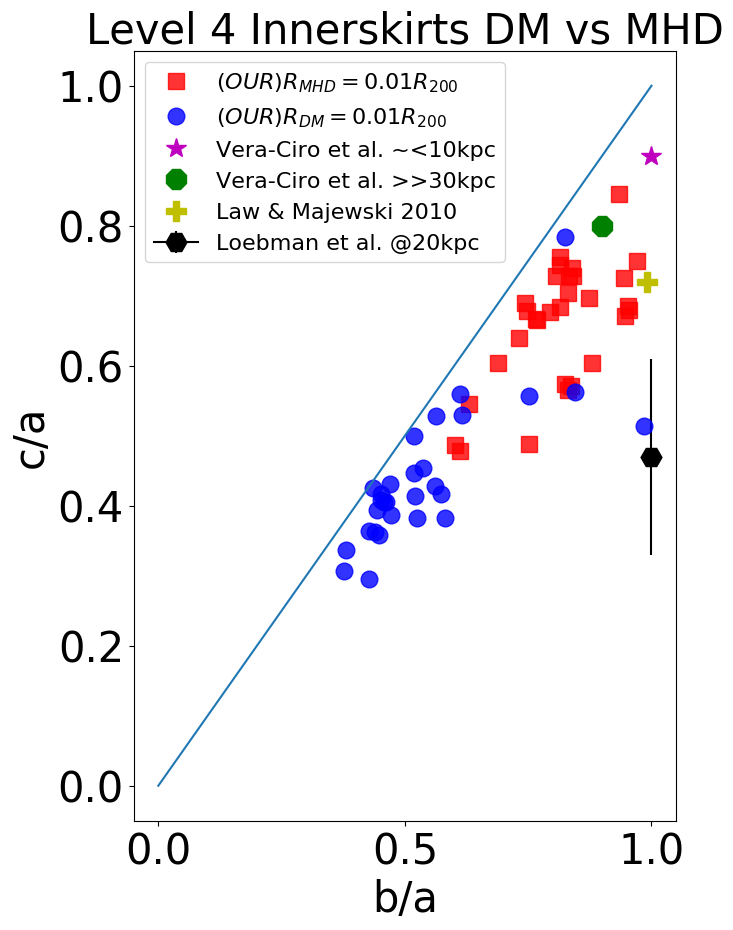
\includegraphics[width=0.5\columnwidth]{./pics/Triaxial_Plane/Triaxiality_Inner_lvl4.png}}
%  \hfill
%  \subfloat[Level4 MHD Vs DM at outer regions]{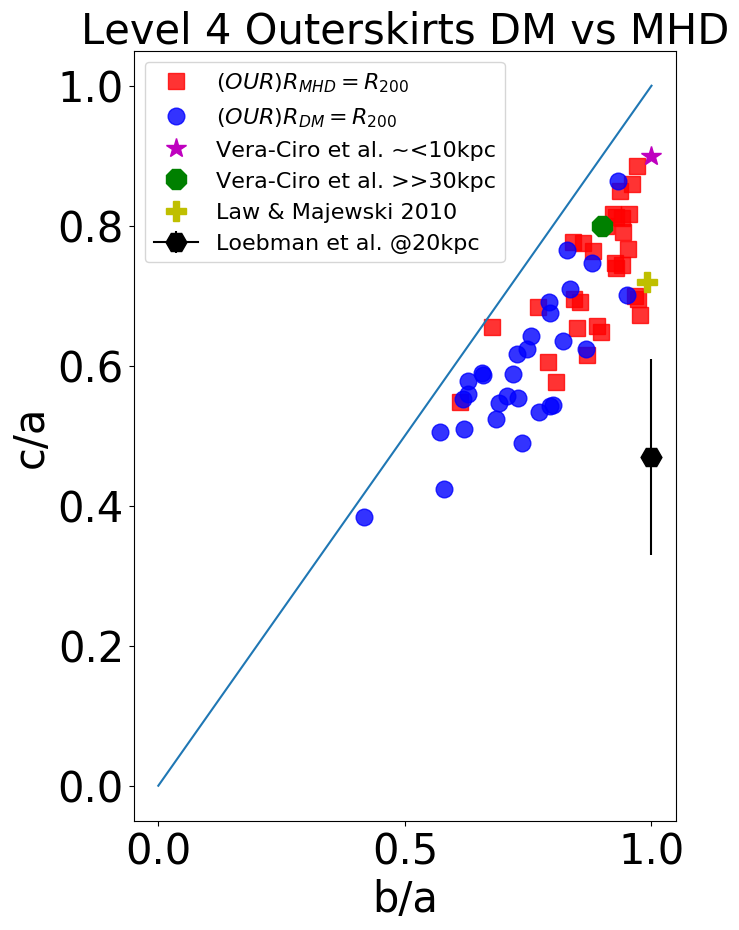
\includegraphics[width=0.5\columnwidth]{./pics/Triaxial_Plane/Triaxiality_Outter_lvl4.png}}
%  \hfill
%  \caption{Axial ratios as shown on $c/a$ Vs $b/a$. Each dot represents a halo shape at some radius. Some observational constraints are plotted alongside our results. Here, dots are clustered, proving the general tendence of halos to get rounder on the outer parts.(Optimize space. caption replaces title.  Present constraints representation of density)}
%  \label{fig:Triaxiality_Inner_Outer}
%\end{figure}


\subsection{The historical shape}
One of the principal motivations to study the radial dependence of the
DM halo shape is that it may encode some clues about its formation
history. We have already shown that DM-only halos seem to exhibit a
steady and monotonous growth in its axial ratios when sampled at
bigger radii. One similar effect can be found if we sample the shape
at the virial radius, this time at varying redshift. It is easy to see
that the axial ratios increase with decreasing redshift, which is
expected by the continuous influence of the gravitational potential
\cite{VeraCiro}. In figure \ref{fig:RedshiftGood} we present a
representative example.  
 
\begin{figure}
  \centering
  \subfloat[halo 16 DM]{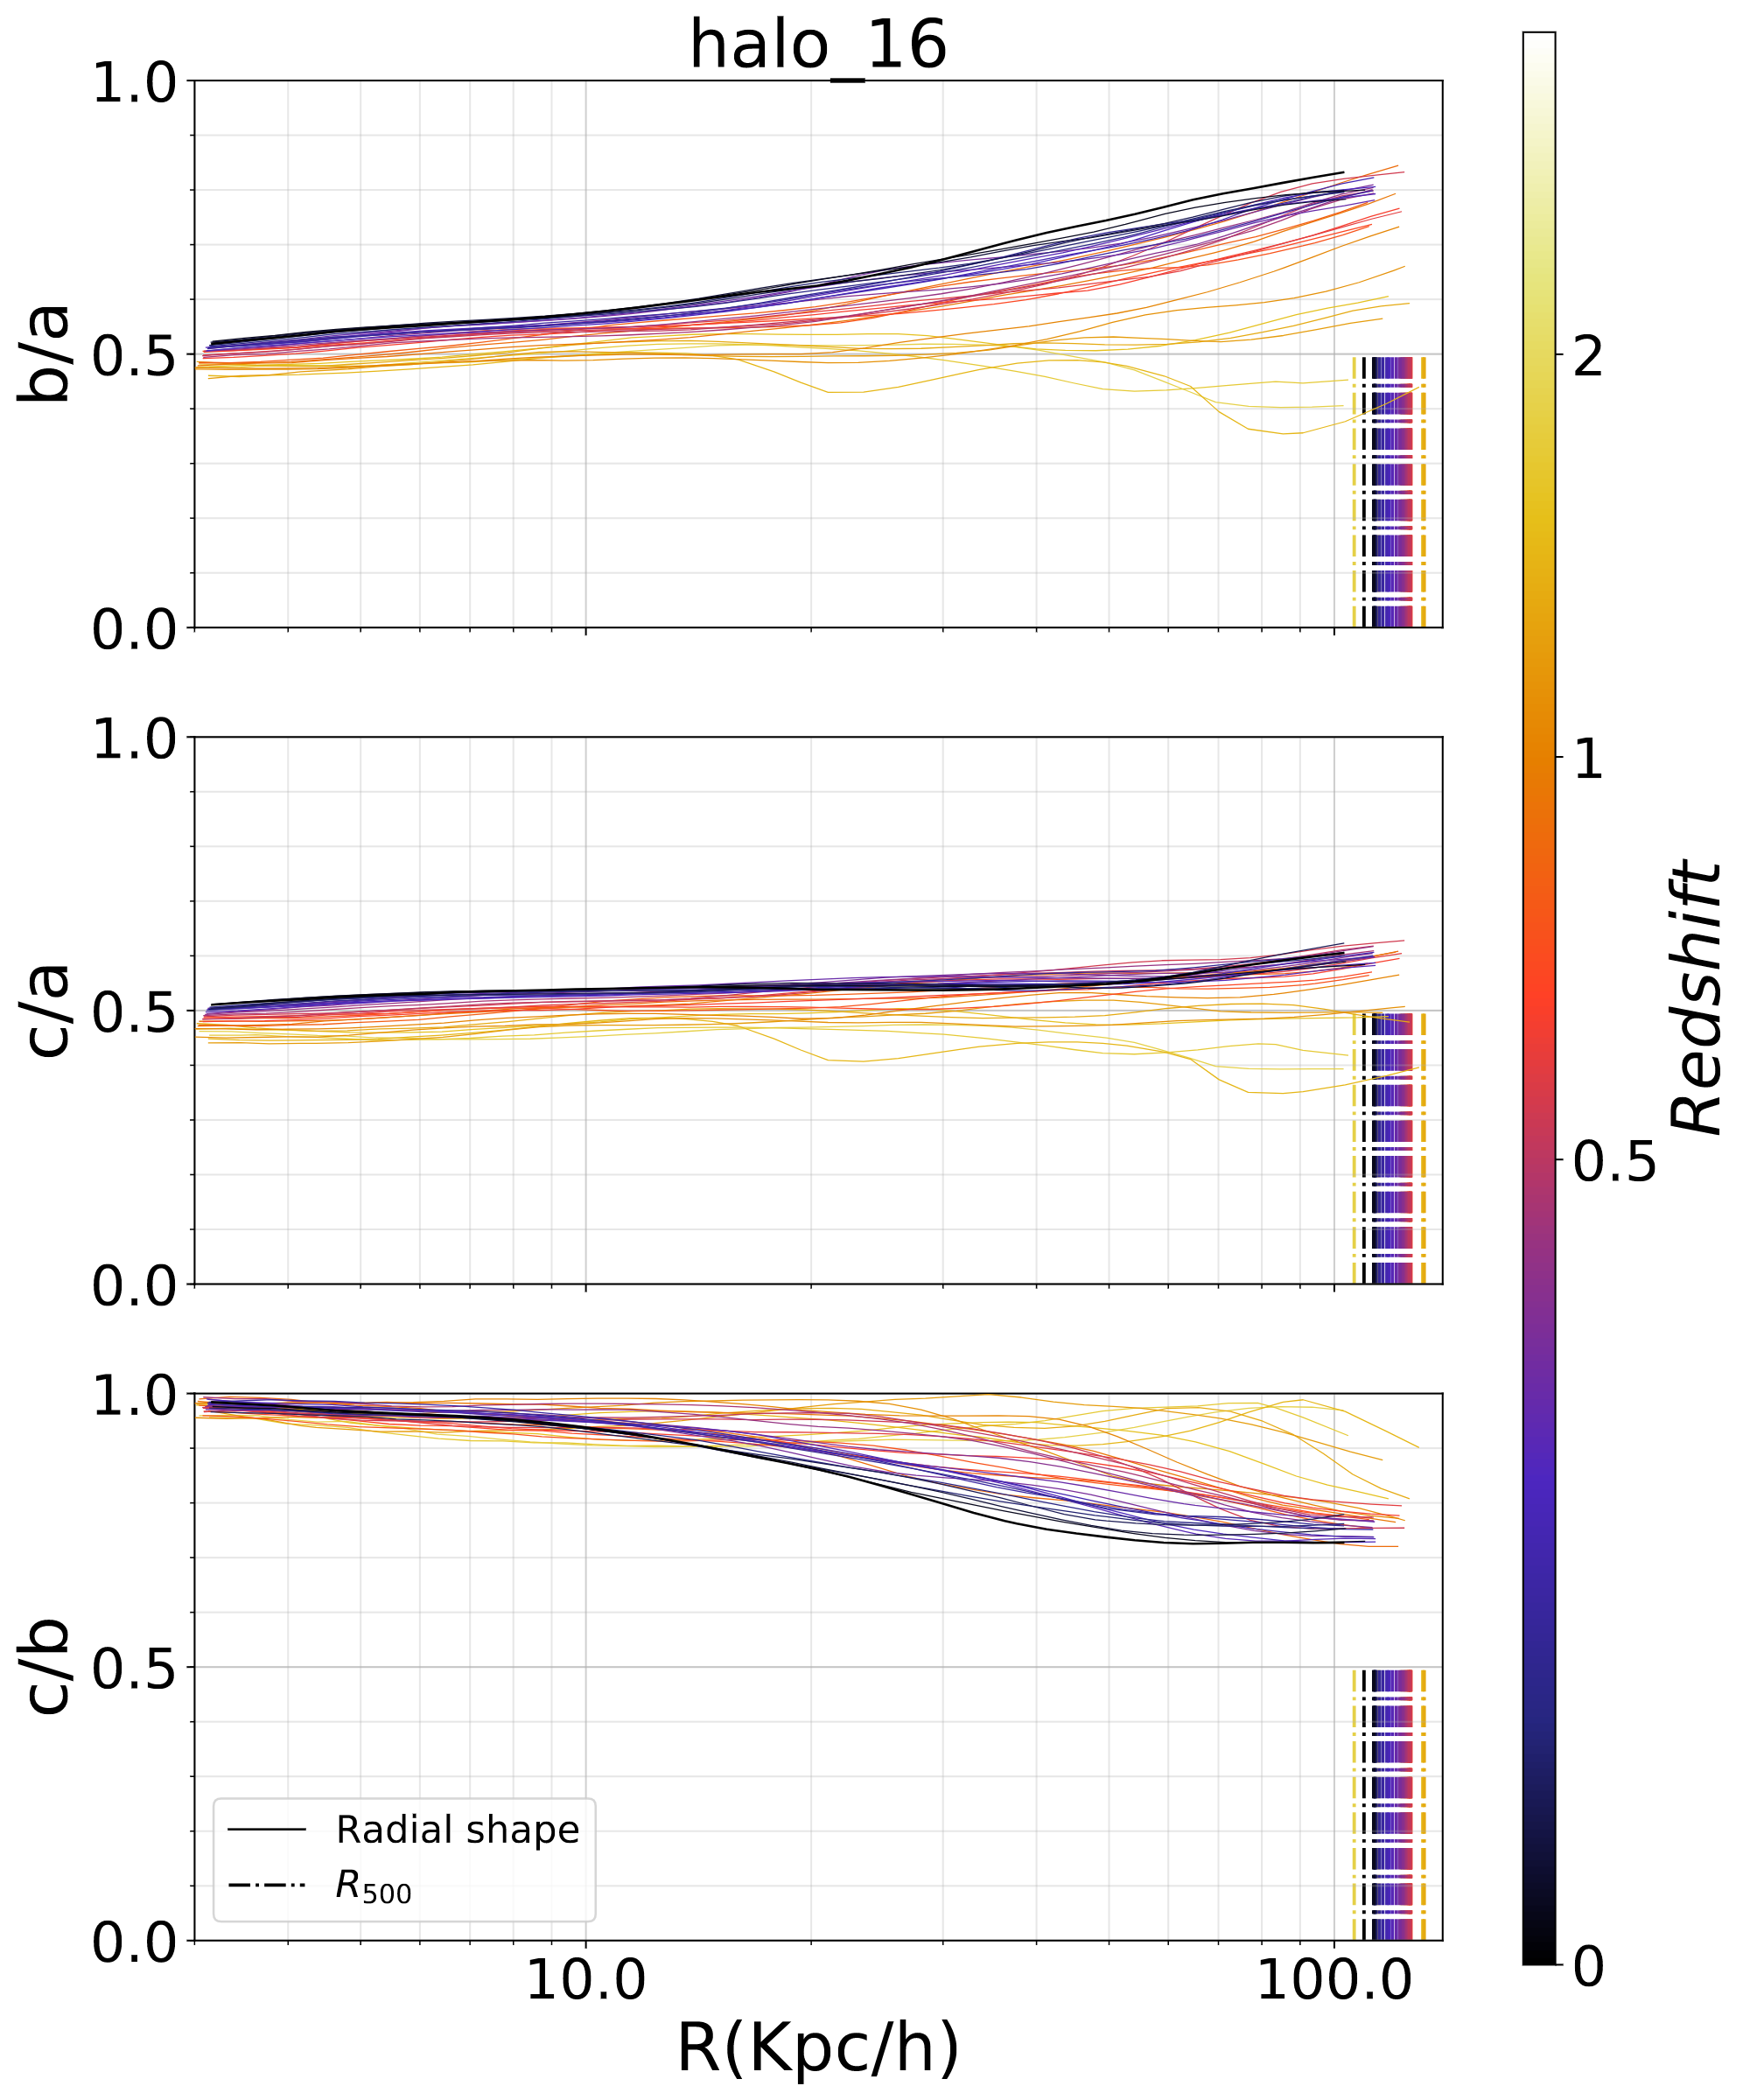
\includegraphics[width=0.5\columnwidth]{./pics/Redshift/halo_16_level3_DM_Z.png}}
  \hfill
  \subfloat[halo 16 MHD]{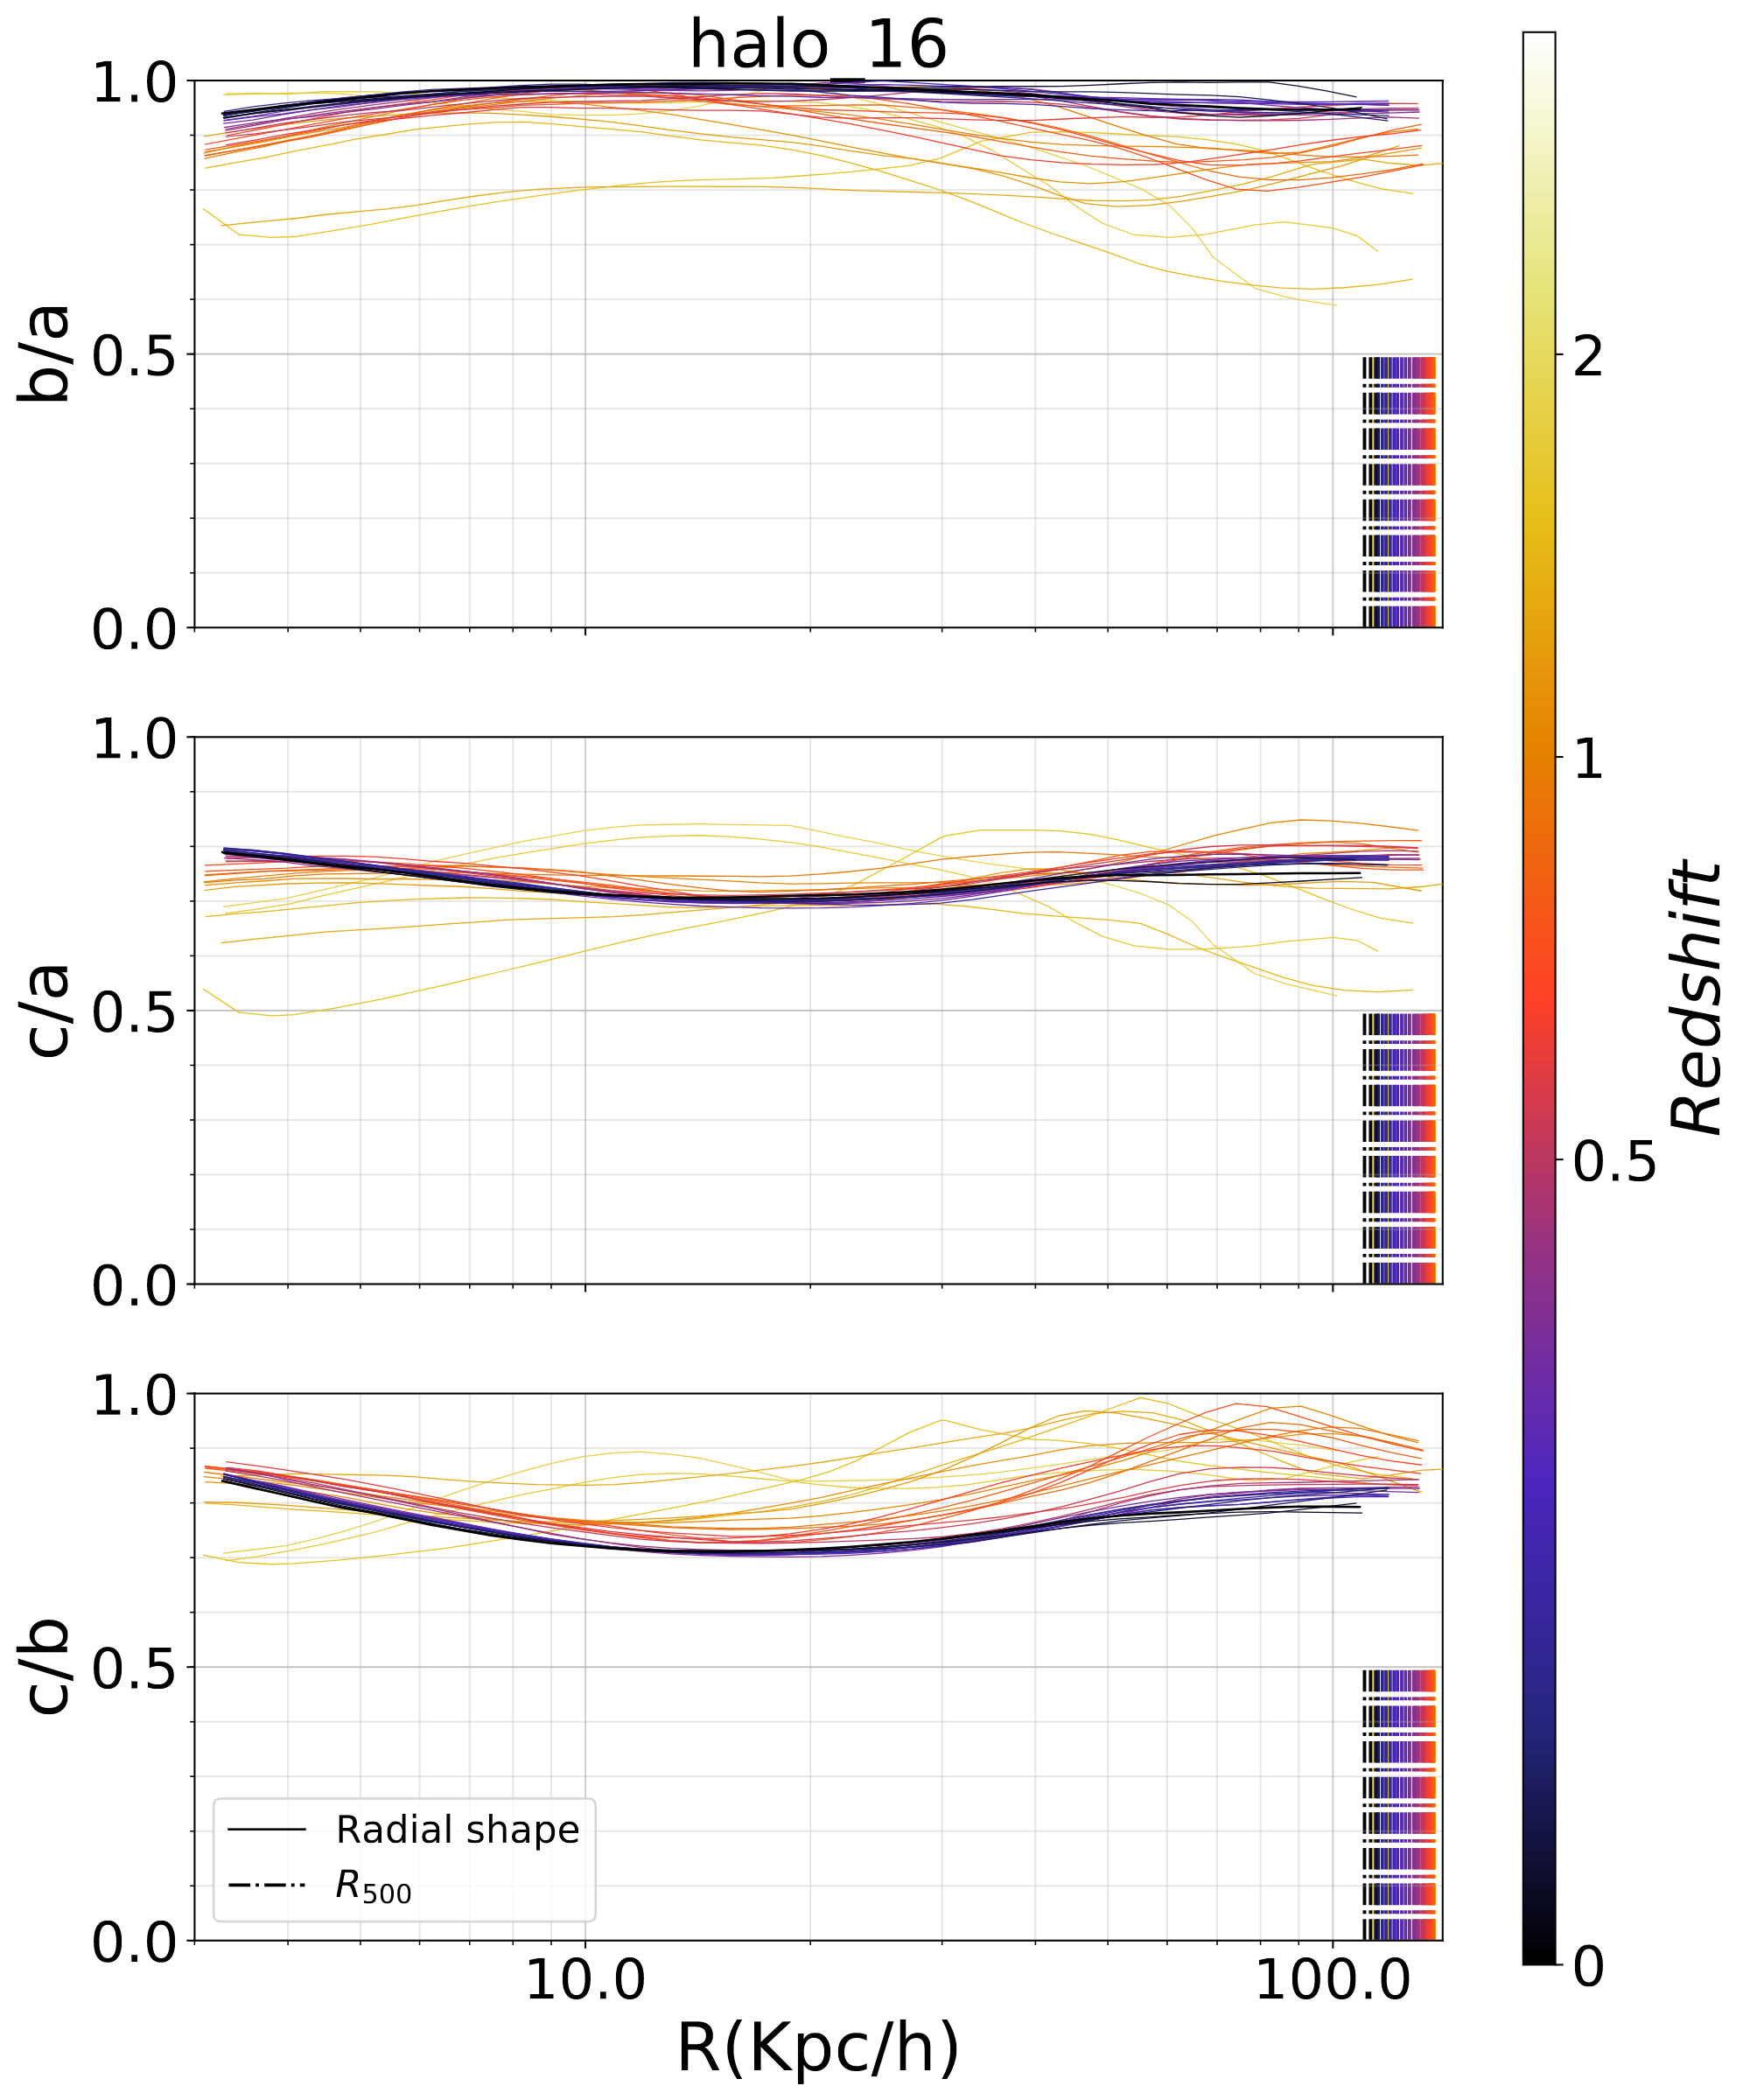
\includegraphics[width=0.5\columnwidth]{./pics/Redshift/halo_16_level3_MHD_Z.png}}
  \caption{Radial profile (comoving) of axial ratios for halo 16 in terms of redshift (color). This halo maintains its shape until $z\approx 1$ obviating the systematic rounding effect in time from asymmetric potentials. }
  \label{fig:RedshiftGood}
\end{figure}


Interestingly, these two parametic plots i.e. $(b/a,c/a)(z=0,r)$ and
$(b/a,c/a)(z,r=R_{vir})$ are very correlated for DM-only halos
\ref{fig:DM Z Triax}. This means that, for DM-only halos, one can
approximate its shape at higher redshift by simply sampling its
current shape at a smaller radius \textbf{wording}. This relationship
relies strongly on the steady and monotonous tendency of DM halos
towards sphericity for bigger radii and smaller redshift. 


\begin{figure}
	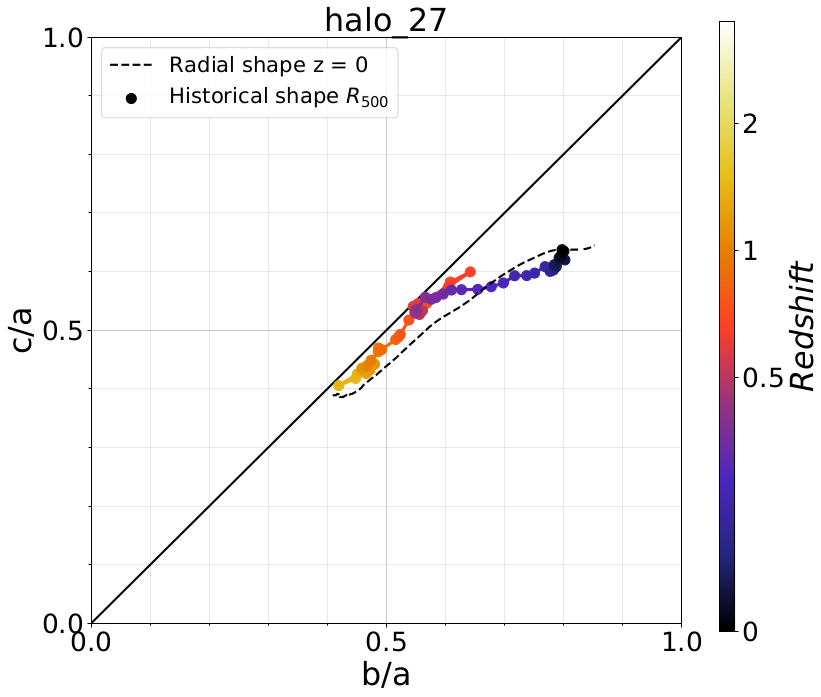
\includegraphics[width=\columnwidth]{./pics/Redshift/halo_27_DM_Z_correlation.png}
    \caption{Difference in asphericities between MHD and DM shapes Vs Star Density of the simulation.}
    \label{fig:DM Z Triax}
    
\end{figure}

MHD halos, on the other hand, do not exhibit tendency towards
sphericity with bigger radii, but they do get sistematically rounder
at lower redshift as seen in figure \ref{fig:RedshiftGood}. This
effectively vanishes this correlation as seen from a DM halo
\ref{fig:MHD Z Triax}. 

\begin{figure}
	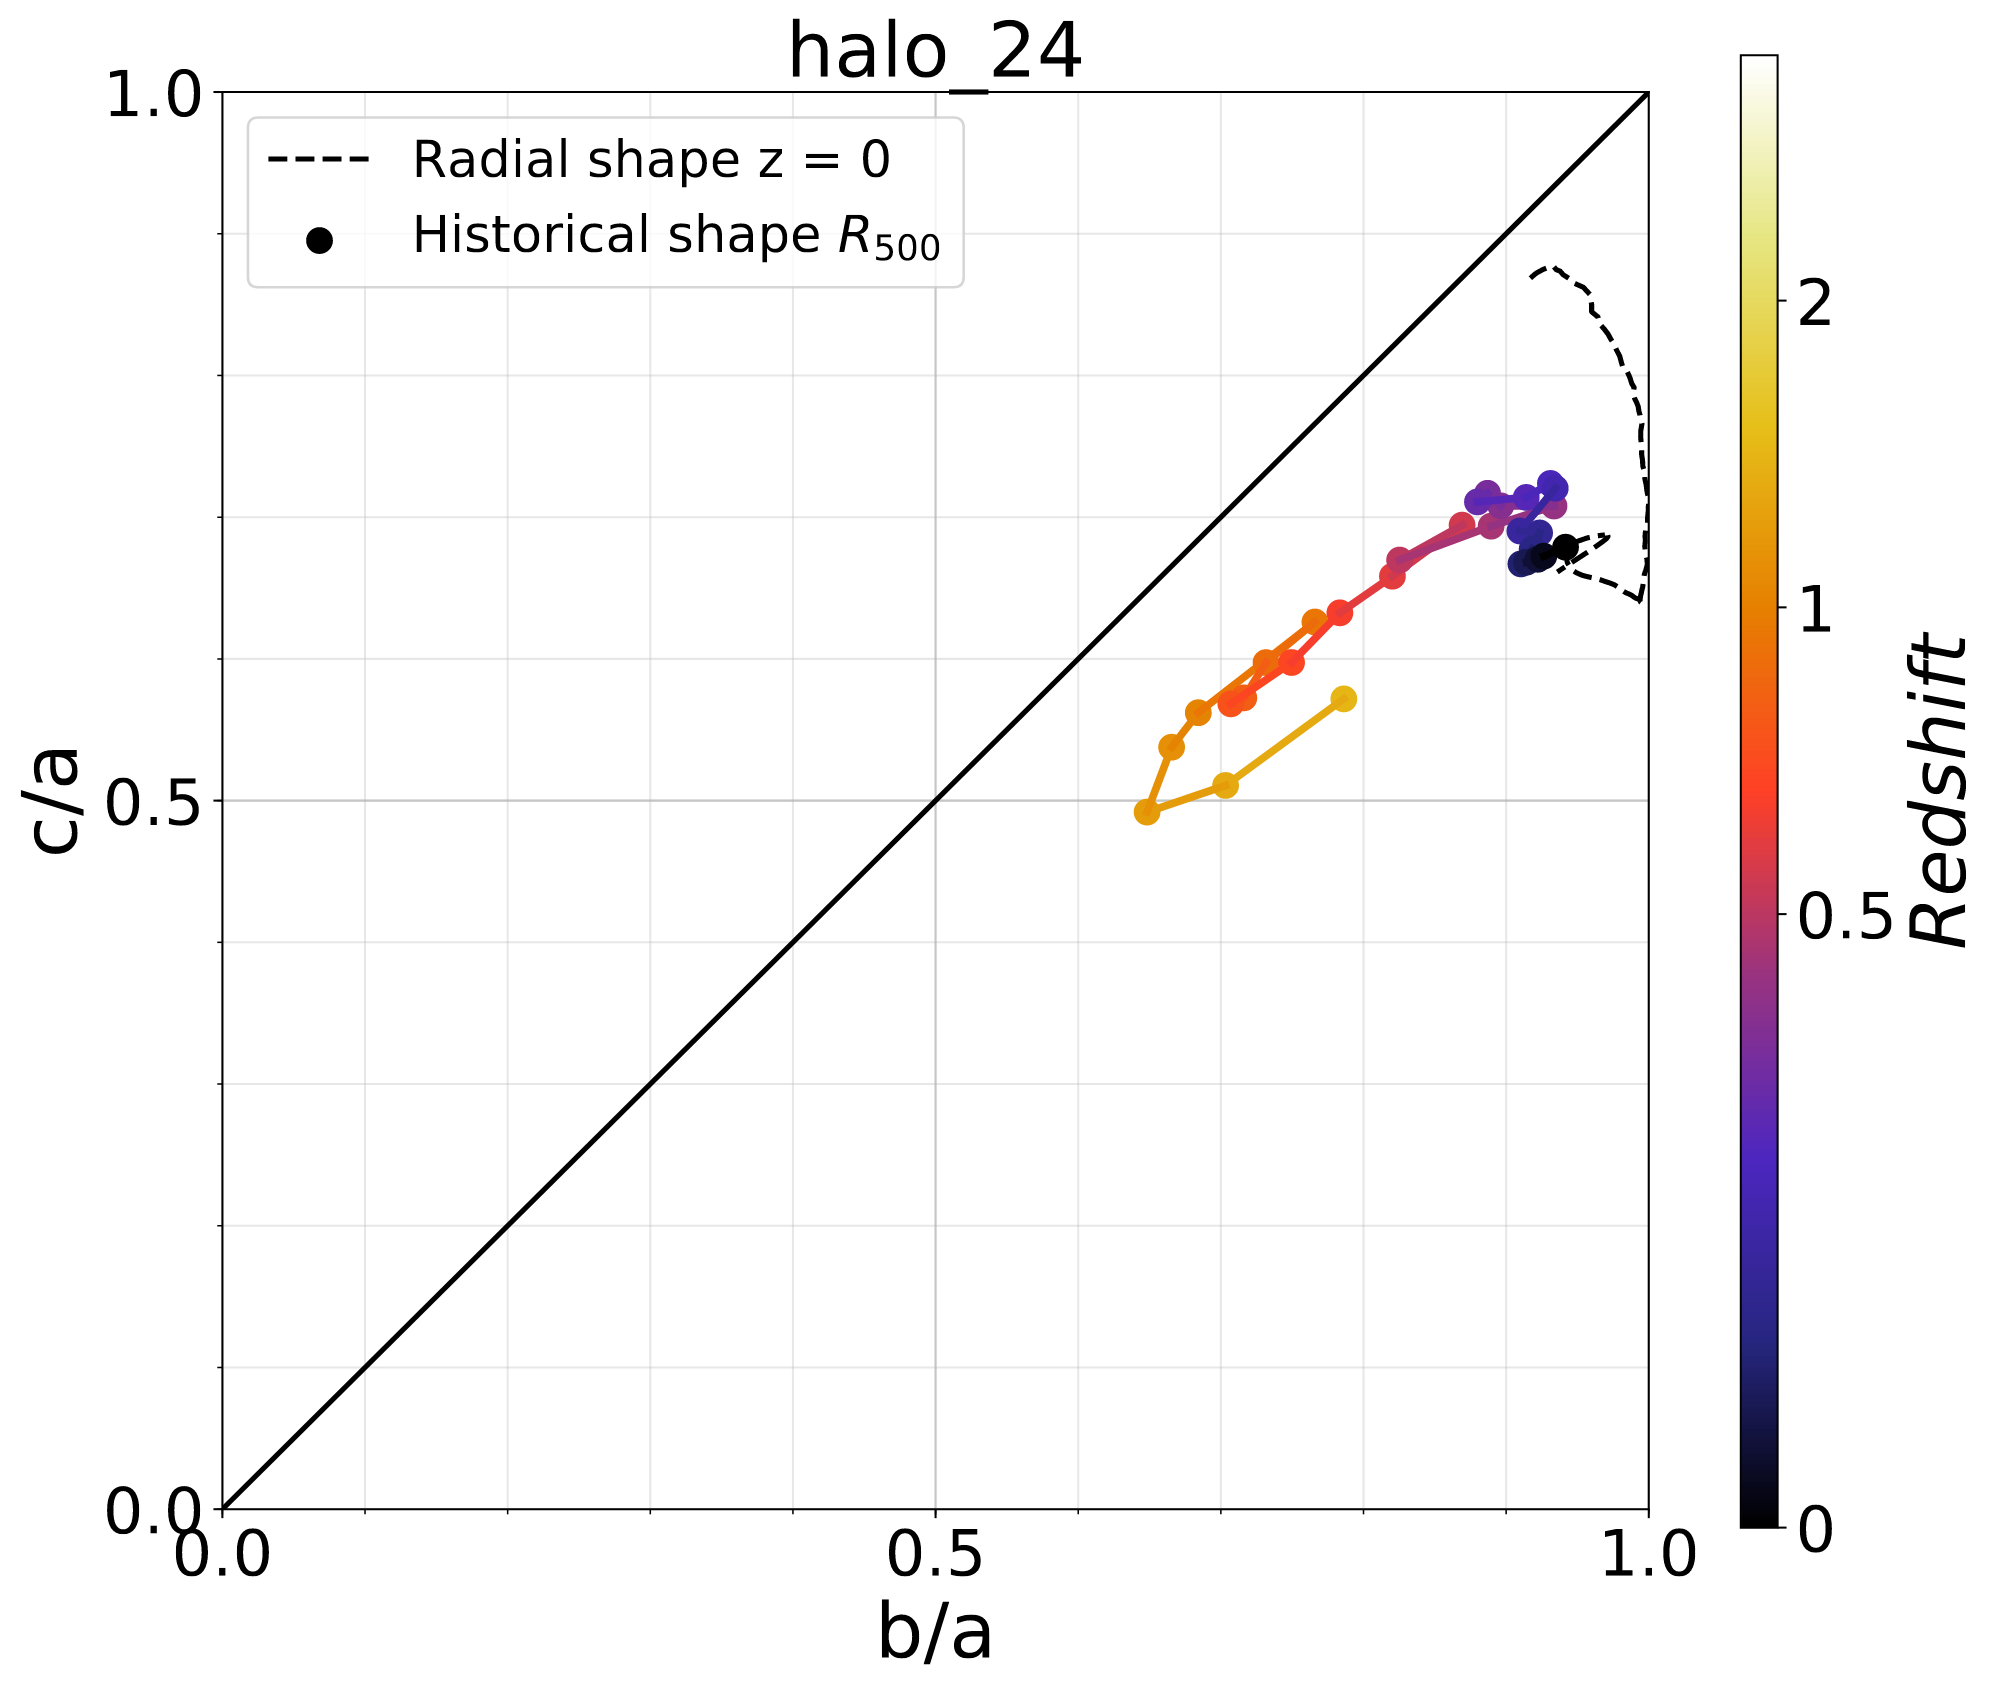
\includegraphics[width=\columnwidth]{./pics/Redshift/halo_24_level3_MHD_Z_Triax.png}
    \caption{Difference in asphericities between MHD and DM shapes Vs
      Star Density of the simulation.} 
    \label{fig:MHD Z Triax} 
\end{figure}

Better graphics.

%Discuss if this correlation may be recovered if compared for example at Disk radius in stead of virial radius.\\


\subsection{The orientation of the principa axes}

One of the principal assumptions of observational models of the MW's
DM halo is that its minor axis is perfectly aligned with the disk
axis. Although this is a reasonable assumption to guarantee the
stability of the galactic disk in simplified models of isolated
galaxies, it may not be the case for galaxies evolved in the whole
cosmological context nor at every radii at which the shape is
sampled. 

Therefore, it is of special interest to us to examin the strength of
this alignment assumption in the context of simulations. For this
purpose, we sampled the shape at 5 different radii and plotted the
axial directions, as well as the disk direction in the \textbf{name}
diagrams \cite{} (explain diagrams). Explain disk direction
calculation. 

We found that there is not a representative example of what happens in
terms of alignments. We found that the majority of the disks are
aligned with the minor axis of their DM halo within $\approx 30^o$; in
some special cases, this alignment was almost perfect and in some
other cases, the DM halo minor axis changed substantially to be able
to determine an alignment. In figure \ref{fig:alignment} we present
these three cases. \textbf{occurrencies for each case?} 


\textit{This is an important result of our study. We study the radial
  evolution of the principal axes, compared also to the angular
  momentum vector from the disk. We found that while the angular
  momentum tend to be aligned with the minor axis of the ellipsoid,
  this may not be the case all times. When there is an alignment it is
  usually within 20 degrees (get a histogram of this. and an evolution
  of this histogram with time). When there is not an alignment, then
  there is no simple way to determine towards which axis it is
  oriented. Furthermore, the principal axes alignment usually change
  with radius (rotation, swap, verify). This ask for relaxation on the
  strong constrains on the MW DM halo models.} 


\begin{figure}
  \centering
  \subfloat[Perfectly aligned Axes]{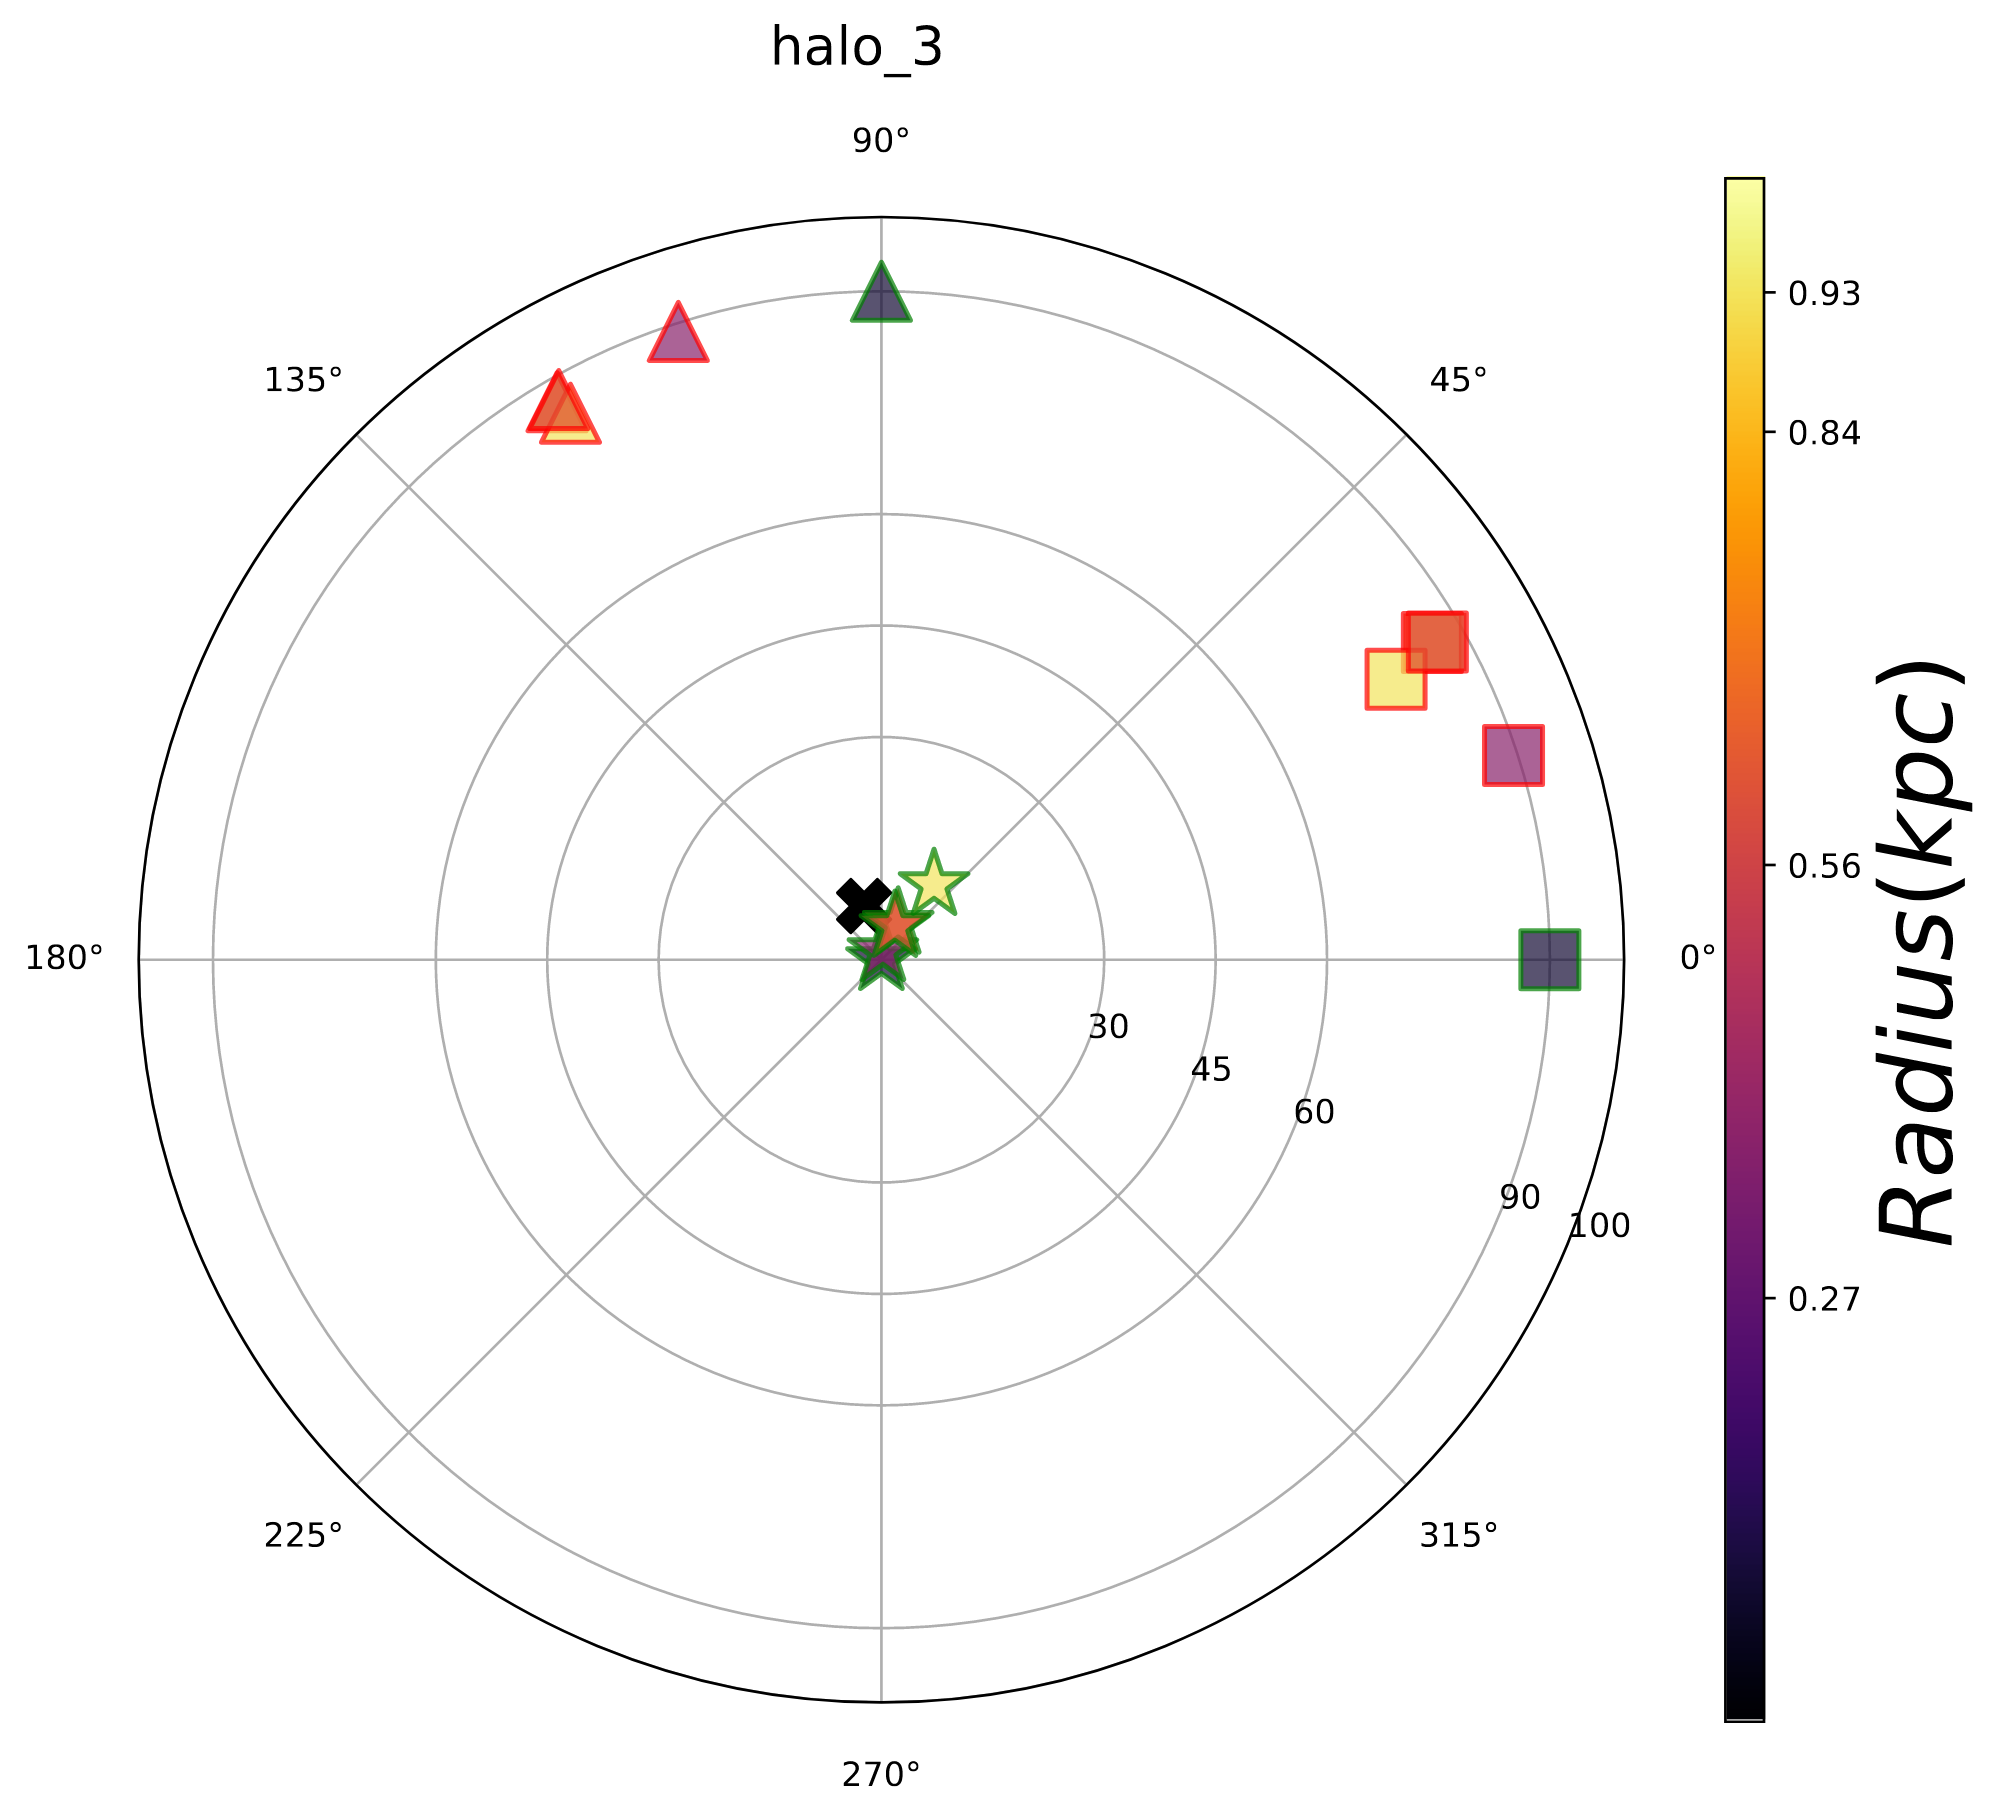
\includegraphics[width=1\columnwidth]{./pics/well_axes.png}}
  \hfill
  \subfloat[Somewhat aligned Axes]{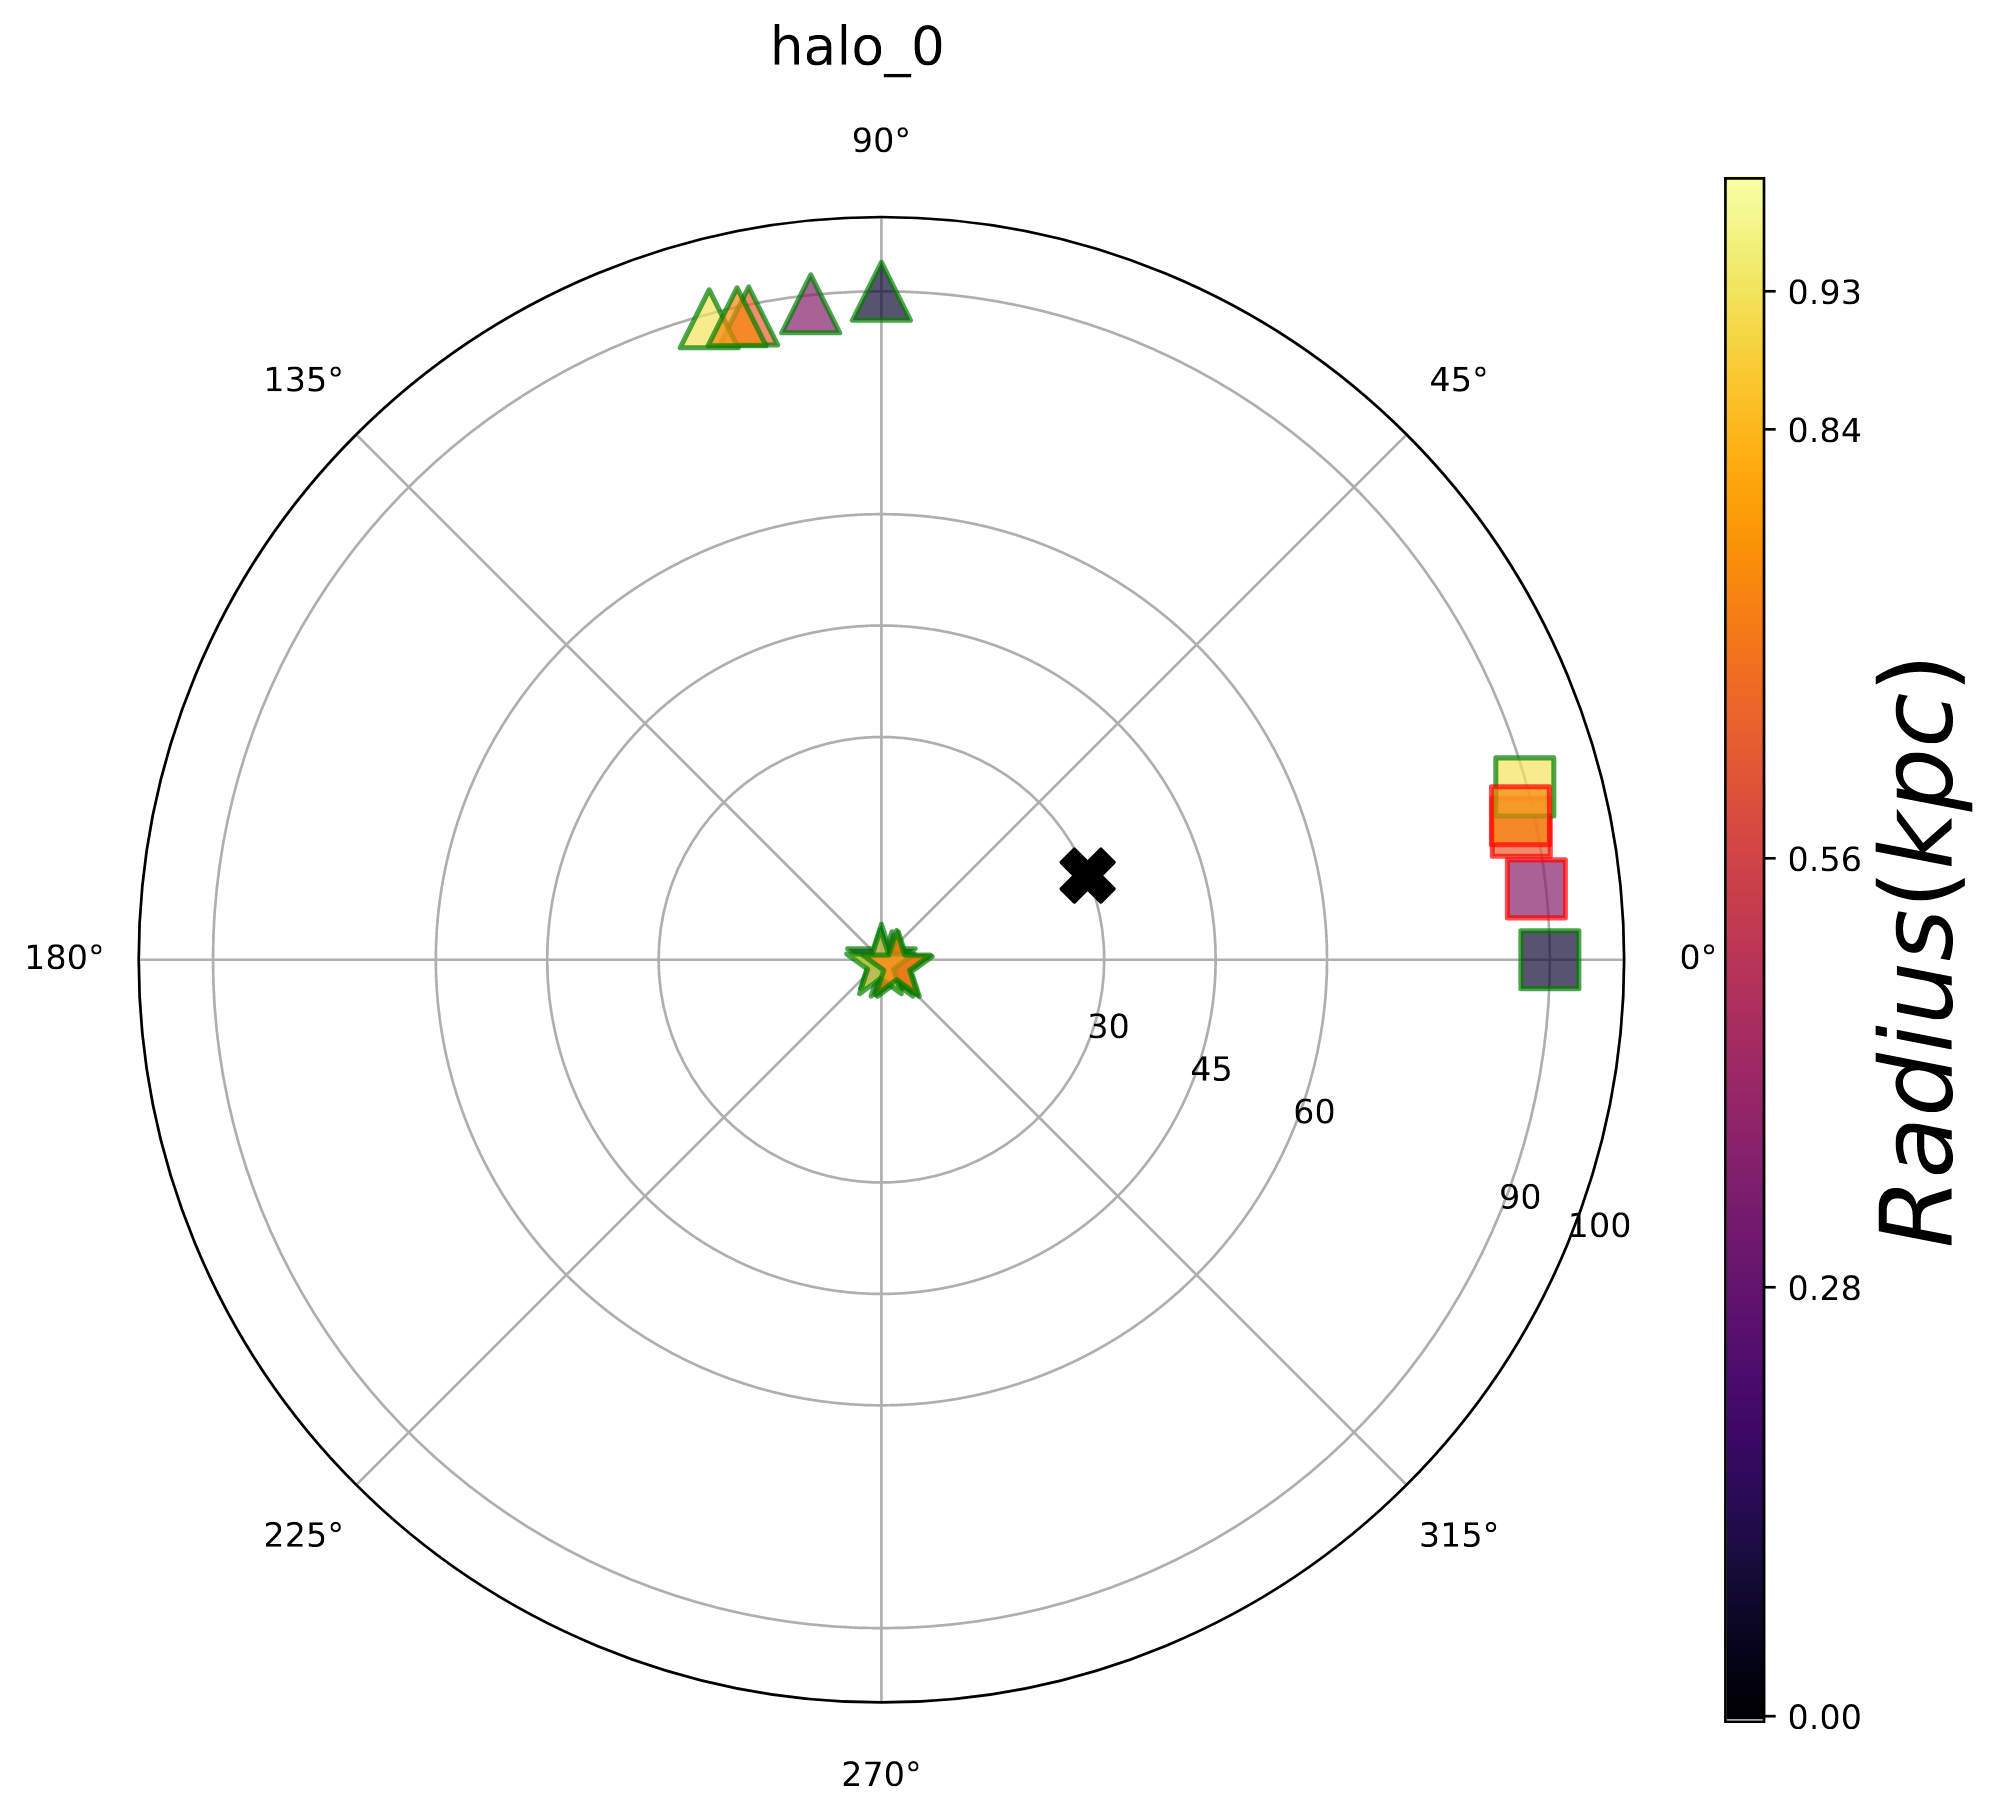
\includegraphics[width=1\columnwidth]{./pics/rotating_axes.png}}
  \hfill
  \subfloat[Chaotic Axes]{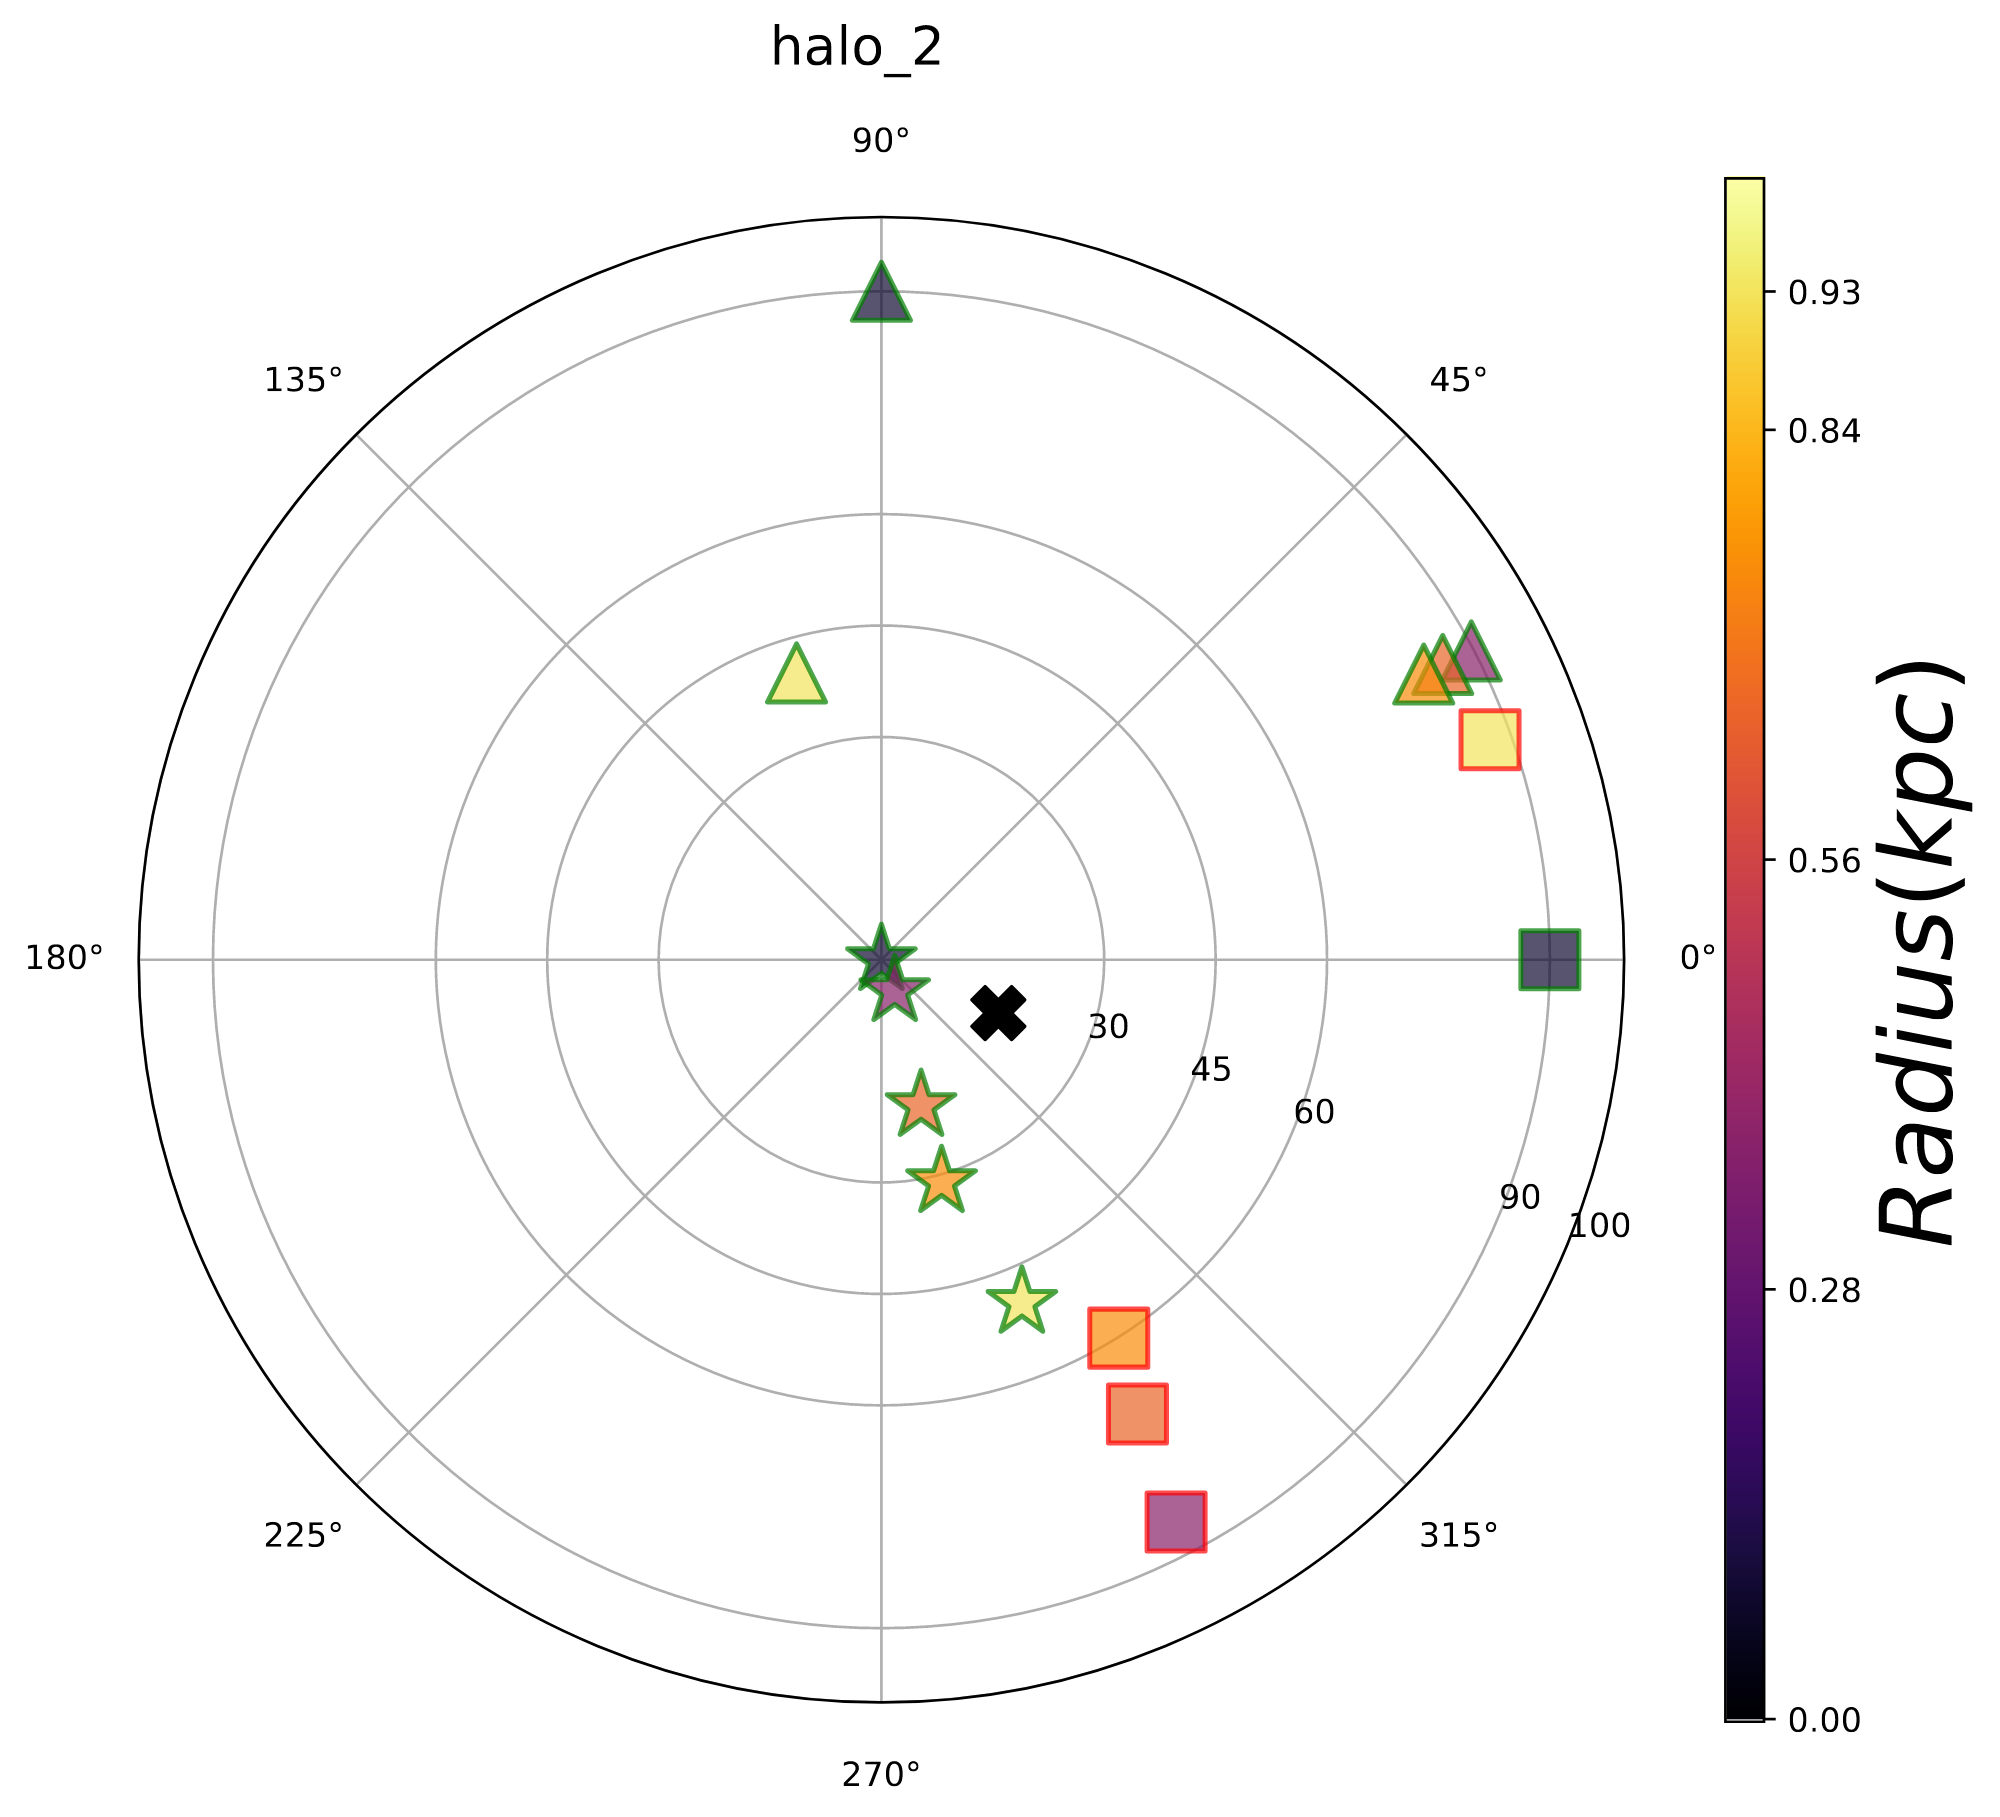
\includegraphics[width=1\columnwidth]{./pics/chaotic_axes.png}}
  \hfill
  \caption{Description of axes alignments }
  \label{fig:alignment}
\end{figure}

\textbf{Discussion about the distribution of alignments and their
  evolution in time: Precesion or temporary instabilities?} 

\section{Conclusions}

\section{Discussion}

\section*{Acknowledgements}
This project has received funding from the European Union’s Horizon
2020 Research and Innovation Programme under the Marie
Sk\l{}odowska-Curie grant agreement No 734374. 


%%%%%%%%%%%%%%%%%%%%%%%%%%%%%%%%%%%%%%%%%%%%%%%%%%

%%%%%%%%%%%%%%%%%%%% REFERENCES %%%%%%%%%%%%%%%%%%

% The best way to enter references is to use BibTeX:



% Alternatively you could enter them by hand, like this:
% This method is tedious and prone to error if you have lots of references
\begin{thebibliography}{99}
\bibitem[\protect\citeauthoryear{Author}{2012}]{Author2012}
Author A.~N., 2013, Journal of Improbable Astronomy, 1, 1
\bibitem[\protect\citeauthoryear{Others}{2013}]{Others2013}
Others S., 2012, Journal of Interesting Stuff, 17, 198
\end{thebibliography}

%%%%%%%%%%%%%%%%%%%%%%%%%%%%%%%%%%%%%%%%%%%%%%%%%%

%%%%%%%%%%%%%%%%% APPENDICES %%%%%%%%%%%%%%%%%%%%%

\appendix

\section{Some extra material}

If you want to present additional material which would interrupt the flow of the main paper,
it can be placed in an Appendix which appears after the list of references.

%%%%%%%%%%%%%%%%%%%%%%%%%%%%%%%%%%%%%%%%%%%%%%%%%%


% Don't change these lines
\bsp	% typesetting comment
\label{lastpage}

\end{document}

% End of mnras_template.tex
